% Generated fragments require trusted human review before compilation.
% This binder never requests shell escape or runs external tools.
\documentclass[11pt]{article}
% Trusted shared apparatus. Requires LuaLaTeX; never use shell escape.
\usepackage{fontspec}
\defaultfontfeatures{Ligatures=TeX}
\IfFontExistsTF{Noto Serif}{\setmainfont{Noto Serif}}{%
  \IfFontExistsTF{DejaVu Serif}{\setmainfont{DejaVu Serif}}{%
    \IfFontExistsTF{Times New Roman}{\setmainfont{Times New Roman}}{%
      \PackageError{gelfand-binder}{No configured Cyrillic serif font installed}{Install Noto Serif or DejaVu Serif, or select an installed Cyrillic font.}%
    }%
  }%
}
\IfFontExistsTF{Noto Sans}{\setsansfont{Noto Sans}}{%
  \IfFontExistsTF{DejaVu Sans}{\setsansfont{DejaVu Sans}}{\setsansfont{Arial}}%
}
\IfFontExistsTF{Noto Sans Mono}{\setmonofont{Noto Sans Mono}}{%
  \IfFontExistsTF{DejaVu Sans Mono}{\setmonofont{DejaVu Sans Mono}}{\setmonofont{Courier New}}%
}
\usepackage[a4paper,margin=22mm]{geometry}
\usepackage{amsmath,amssymb,amsthm,mathtools}
\usepackage{xcolor}
\usepackage{tikz}
\usepackage{tikz-cd}
\usetikzlibrary{arrows.meta,positioning,calc}
\usepackage{hyperref}
\hypersetup{unicode=true,colorlinks=true,linkcolor=blue,pdftitle={Gelfand transcription binder}}
\newtheorem{theorem}{Theorem}
\newtheorem{lemma}{Lemma}
\newtheorem{proposition}{Proposition}
\newtheorem{corollary}{Corollary}
\theoremstyle{definition}
\newtheorem{definition}{Definition}
\newtheorem{example}{Example}
\theoremstyle{remark}
\newtheorem{remark}{Remark}
\setlength{\parindent}{0pt}
\setlength{\parskip}{0.55em}
\setlength{\emergencystretch}{3em}
\newcommand{\SourcePage}[2]{%
  \clearpage\phantomsection\label{#1:source-page}%
  \addcontentsline{toc}{subsection}{#1}%
  {\small\sffamily\color{blue!60!black}Source scan frame: #1; visible page/leaf label: #2}\par\medskip%
}
\newcommand{\Unclear}[3]{%
  \begingroup\color{orange!70!black}%
  [Unresolved reading #1/#2: #3]\endgroup%
}
\newcommand{\Incomplete}[3]{%
  \par\begingroup\color{red!65!black}\textbf{Incomplete #1/#2:} #3\endgroup\par%
}
\newcommand{\SourceFigure}[3]{%
  \par\begingroup\color{blue!60!black}\textbf{\hyperref[#1:source-page]{Source figure #1/#2}:} #3%
  \par\textit{Consult the authoritative scan at this locator.}\endgroup\par%
}



% Reader layout only. Original diplomatic text is retained verbatim.
\setlength{\parskip}{0.35em}
\setlength{\emergencystretch}{4em}
\renewcommand{\SourcePage}[2]{%
  \par\addvspace{1em}\phantomsection\label{#1:source-page}%
  \addcontentsline{toc}{subsection}{#1}%
  {\footnotesize\sffamily\color{blue!55!black}#1%
    \def\givenlabel{#2}\def\nolabel{unlabelled}%
    \ifx\givenlabel\nolabel\else\quad[номер в источнике: #2]\fi
  }\par\nobreak\smallskip%
}
\renewcommand{\Unclear}[3]{%
  \begingroup\color{orange!65!black}%
  \ifmmode\text{[неясно: #3]}\else[неясно: #3]\fi\endgroup%
}
\renewcommand{\Incomplete}[3]{%
  \par\begingroup\color{red!60!black}\textbf{Неразобранный фрагмент:} #3%
  \endgroup\par%
}
\renewcommand{\SourceFigure}[3]{%
  \par\begingroup\color{blue!55!black}\textbf{Рисунок:} #3%
  \par{\small\textit{Исходный рисунок: \hyperref[#1:source-page]{#1}, #2.}}%
  \endgroup\par%
}
\hypersetup{pdftitle={Семинар И. М. Гельфанда. Дипломатическая транскрипция},pdfauthor={},pdfsubject={Русское рабочее издание с отмеченными сомнительными чтениями}}

\usepackage[normalem]{ulem}
\usepackage{newunicodechar}
\usepackage{adjustbox}
\newfontfamily\SourceSymbolFont{Segoe UI Symbol}
\newfontfamily\SourceCJKFont{MS Gothic}
\let\DiplomaticMathUnderline\underline
\renewcommand{\underline}[1]{\ifmmode\DiplomaticMathUnderline{#1}\else\uline{#1}\fi}
\newunicodechar{→}{\ifmmode\text{{\SourceSymbolFont\char"2192}}\else{\SourceSymbolFont\char"2192}\fi}
\newunicodechar{⇒}{\ifmmode\text{{\SourceSymbolFont\char"21D2}}\else{\SourceSymbolFont\char"21D2}\fi}
\newunicodechar{∀}{\ifmmode\text{{\SourceSymbolFont\char"2200}}\else{\SourceSymbolFont\char"2200}\fi}
\newunicodechar{∂}{\ifmmode\text{{\SourceSymbolFont\char"2202}}\else{\SourceSymbolFont\char"2202}\fi}
\newunicodechar{∈}{\ifmmode\text{{\SourceSymbolFont\char"2208}}\else{\SourceSymbolFont\char"2208}\fi}
\newunicodechar{∌}{\ifmmode\text{{\SourceSymbolFont\char"220C}}\else{\SourceSymbolFont\char"220C}\fi}
\newunicodechar{√}{\ifmmode\text{{\SourceSymbolFont\char"221A}}\else{\SourceSymbolFont\char"221A}\fi}
\newunicodechar{∞}{\ifmmode\text{{\SourceSymbolFont\char"221E}}\else{\SourceSymbolFont\char"221E}\fi}
\newunicodechar{∧}{\ifmmode\text{{\SourceSymbolFont\char"2227}}\else{\SourceSymbolFont\char"2227}\fi}
\newunicodechar{∩}{\ifmmode\text{{\SourceSymbolFont\char"2229}}\else{\SourceSymbolFont\char"2229}\fi}
\newunicodechar{∪}{\ifmmode\text{{\SourceSymbolFont\char"222A}}\else{\SourceSymbolFont\char"222A}\fi}
\newunicodechar{∫}{\ifmmode\text{{\SourceSymbolFont\char"222B}}\else{\SourceSymbolFont\char"222B}\fi}
\newunicodechar{∴}{\ifmmode\text{{\SourceSymbolFont\char"2234}}\else{\SourceSymbolFont\char"2234}\fi}
\newunicodechar{∼}{\ifmmode\text{{\SourceSymbolFont\char"223C}}\else{\SourceSymbolFont\char"223C}\fi}
\newunicodechar{≈}{\ifmmode\text{{\SourceSymbolFont\char"2248}}\else{\SourceSymbolFont\char"2248}\fi}
\newunicodechar{≠}{\ifmmode\text{{\SourceSymbolFont\char"2260}}\else{\SourceSymbolFont\char"2260}\fi}
\newunicodechar{≤}{\ifmmode\text{{\SourceSymbolFont\char"2264}}\else{\SourceSymbolFont\char"2264}\fi}
\newunicodechar{≥}{\ifmmode\text{{\SourceSymbolFont\char"2265}}\else{\SourceSymbolFont\char"2265}\fi}
\newunicodechar{⊕}{\ifmmode\text{{\SourceSymbolFont\char"2295}}\else{\SourceSymbolFont\char"2295}\fi}
\newunicodechar{⊗}{\ifmmode\text{{\SourceSymbolFont\char"2297}}\else{\SourceSymbolFont\char"2297}\fi}
\newunicodechar{①}{\ifmmode\text{{\SourceSymbolFont\char"2460}}\else{\SourceSymbolFont\char"2460}\fi}
\newunicodechar{②}{\ifmmode\text{{\SourceSymbolFont\char"2461}}\else{\SourceSymbolFont\char"2461}\fi}
\newunicodechar{③}{\ifmmode\text{{\SourceSymbolFont\char"2462}}\else{\SourceSymbolFont\char"2462}\fi}
\newunicodechar{④}{\ifmmode\text{{\SourceSymbolFont\char"2463}}\else{\SourceSymbolFont\char"2463}\fi}
\newunicodechar{Ⓗ}{\ifmmode\text{{\SourceSymbolFont\char"24BD}}\else{\SourceSymbolFont\char"24BD}\fi}
\newunicodechar{〃}{\ifmmode\text{{\SourceCJKFont\char"3003}}\else{\SourceCJKFont\char"3003}\fi}


% Reader revision 3. Annotation wording and candidates remain unchanged.
\setmainfont{NotoSerif-Regular.ttf}[Path=C:/Windows/Fonts/,ItalicFont=NotoSerif-Italic.ttf,BoldFont=NotoSerif-Bold.ttf,BoldItalicFont=NotoSerif-BoldItalic.ttf]
\usetikzlibrary{shapes.geometric,decorations.pathreplacing,decorations.markings,patterns,fit}
\newsavebox{\ReaderAnnotationBox}
\newcommand{\ReaderAnnotation}[1]{%
  \sbox{\ReaderAnnotationBox}{[неясно: #1]}%
  \ifdim\wd\ReaderAnnotationBox>.70\linewidth
    \parbox[t]{.70\linewidth}{\raggedright[неясно: #1]}%
  \else\usebox{\ReaderAnnotationBox}\fi%
}
\ExplSyntaxOn
\cs_new_protected:Npn \reader_unclear_candidate:n #1
 {
  \tl_set:Nx \l_tmpa_tl { \tl_to_str:n {#1} }
  % Text explicitly guarded inside a mathematical candidate remains math-safe.
  \regex_replace_all:nnN { \\(?:text|textrm|textnormal|textbf|operatorname)\s*\{[^{}]*\} } { } \l_tmpa_tl
  \regex_match:nVTF { [\x{0400}-\x{052F}] | \$ } \l_tmpa_tl
   { \ifmmode \text{\ReaderAnnotation{#1}} \else \ReaderAnnotation{#1} \fi }
   {
    \ifmmode
      [\text{неясно:~}#1]
    \else
      \regex_match:nVTF { [_^] | \\ } \l_tmpa_tl
       { \ensuremath{[\text{неясно:~}#1]} }
       { \ReaderAnnotation{#1} }
    \fi
   }
 }
\RenewDocumentCommand \Unclear { m m m }
 { \begingroup\color{orange!65!black}\reader_unclear_candidate:n{#3}\endgroup }
\ExplSyntaxOff
\newsavebox{\ReaderIncompleteBox}
\newcommand{\ReaderIncompleteNote}[1]{%
 \sbox{\ReaderIncompleteBox}{\textbf{Неразобранный фрагмент:} #1}%
 \ifdim\wd\ReaderIncompleteBox>.70\linewidth
  \parbox[t]{.70\linewidth}{\raggedright\textbf{Неразобранный фрагмент:} #1}%
 \else\usebox{\ReaderIncompleteBox}\fi%
}
\renewcommand{\Incomplete}[3]{%
 \ifmmode\text{\color{red!60!black}\ReaderIncompleteNote{#3}}%
 \else\leavevmode\begingroup\color{red!60!black}\ReaderIncompleteNote{#3}\endgroup\fi%
}
% Ragged right avoids stretching long untranslated abbreviations into margins.
\AtBeginDocument{\raggedright}
\newunicodechar{А}{\ifmmode\text{\char"410\relax}\else\char"410\relax\fi}
\newunicodechar{Б}{\ifmmode\text{\char"411\relax}\else\char"411\relax\fi}
\newunicodechar{В}{\ifmmode\text{\char"412\relax}\else\char"412\relax\fi}
\newunicodechar{Г}{\ifmmode\text{\char"413\relax}\else\char"413\relax\fi}
\newunicodechar{Д}{\ifmmode\text{\char"414\relax}\else\char"414\relax\fi}
\newunicodechar{Е}{\ifmmode\text{\char"415\relax}\else\char"415\relax\fi}
\newunicodechar{Ж}{\ifmmode\text{\char"416\relax}\else\char"416\relax\fi}
\newunicodechar{З}{\ifmmode\text{\char"417\relax}\else\char"417\relax\fi}
\newunicodechar{И}{\ifmmode\text{\char"418\relax}\else\char"418\relax\fi}
\newunicodechar{Й}{\ifmmode\text{\char"419\relax}\else\char"419\relax\fi}
\newunicodechar{К}{\ifmmode\text{\char"41A\relax}\else\char"41A\relax\fi}
\newunicodechar{Л}{\ifmmode\text{\char"41B\relax}\else\char"41B\relax\fi}
\newunicodechar{М}{\ifmmode\text{\char"41C\relax}\else\char"41C\relax\fi}
\newunicodechar{Н}{\ifmmode\text{\char"41D\relax}\else\char"41D\relax\fi}
\newunicodechar{О}{\ifmmode\text{\char"41E\relax}\else\char"41E\relax\fi}
\newunicodechar{П}{\ifmmode\text{\char"41F\relax}\else\char"41F\relax\fi}
\newunicodechar{Р}{\ifmmode\text{\char"420\relax}\else\char"420\relax\fi}
\newunicodechar{С}{\ifmmode\text{\char"421\relax}\else\char"421\relax\fi}
\newunicodechar{Т}{\ifmmode\text{\char"422\relax}\else\char"422\relax\fi}
\newunicodechar{У}{\ifmmode\text{\char"423\relax}\else\char"423\relax\fi}
\newunicodechar{Ф}{\ifmmode\text{\char"424\relax}\else\char"424\relax\fi}
\newunicodechar{Х}{\ifmmode\text{\char"425\relax}\else\char"425\relax\fi}
\newunicodechar{Ц}{\ifmmode\text{\char"426\relax}\else\char"426\relax\fi}
\newunicodechar{Ч}{\ifmmode\text{\char"427\relax}\else\char"427\relax\fi}
\newunicodechar{Ш}{\ifmmode\text{\char"428\relax}\else\char"428\relax\fi}
\newunicodechar{Щ}{\ifmmode\text{\char"429\relax}\else\char"429\relax\fi}
\newunicodechar{Ъ}{\ifmmode\text{\char"42A\relax}\else\char"42A\relax\fi}
\newunicodechar{Ы}{\ifmmode\text{\char"42B\relax}\else\char"42B\relax\fi}
\newunicodechar{Ь}{\ifmmode\text{\char"42C\relax}\else\char"42C\relax\fi}
\newunicodechar{Э}{\ifmmode\text{\char"42D\relax}\else\char"42D\relax\fi}
\newunicodechar{Ю}{\ifmmode\text{\char"42E\relax}\else\char"42E\relax\fi}
\newunicodechar{Я}{\ifmmode\text{\char"42F\relax}\else\char"42F\relax\fi}
\newunicodechar{а}{\ifmmode\text{\char"430\relax}\else\char"430\relax\fi}
\newunicodechar{б}{\ifmmode\text{\char"431\relax}\else\char"431\relax\fi}
\newunicodechar{в}{\ifmmode\text{\char"432\relax}\else\char"432\relax\fi}
\newunicodechar{г}{\ifmmode\text{\char"433\relax}\else\char"433\relax\fi}
\newunicodechar{д}{\ifmmode\text{\char"434\relax}\else\char"434\relax\fi}
\newunicodechar{е}{\ifmmode\text{\char"435\relax}\else\char"435\relax\fi}
\newunicodechar{ж}{\ifmmode\text{\char"436\relax}\else\char"436\relax\fi}
\newunicodechar{з}{\ifmmode\text{\char"437\relax}\else\char"437\relax\fi}
\newunicodechar{и}{\ifmmode\text{\char"438\relax}\else\char"438\relax\fi}
\newunicodechar{й}{\ifmmode\text{\char"439\relax}\else\char"439\relax\fi}
\newunicodechar{к}{\ifmmode\text{\char"43A\relax}\else\char"43A\relax\fi}
\newunicodechar{л}{\ifmmode\text{\char"43B\relax}\else\char"43B\relax\fi}
\newunicodechar{м}{\ifmmode\text{\char"43C\relax}\else\char"43C\relax\fi}
\newunicodechar{н}{\ifmmode\text{\char"43D\relax}\else\char"43D\relax\fi}
\newunicodechar{о}{\ifmmode\text{\char"43E\relax}\else\char"43E\relax\fi}
\newunicodechar{п}{\ifmmode\text{\char"43F\relax}\else\char"43F\relax\fi}
\newunicodechar{р}{\ifmmode\text{\char"440\relax}\else\char"440\relax\fi}
\newunicodechar{с}{\ifmmode\text{\char"441\relax}\else\char"441\relax\fi}
\newunicodechar{т}{\ifmmode\text{\char"442\relax}\else\char"442\relax\fi}
\newunicodechar{у}{\ifmmode\text{\char"443\relax}\else\char"443\relax\fi}
\newunicodechar{ф}{\ifmmode\text{\char"444\relax}\else\char"444\relax\fi}
\newunicodechar{х}{\ifmmode\text{\char"445\relax}\else\char"445\relax\fi}
\newunicodechar{ц}{\ifmmode\text{\char"446\relax}\else\char"446\relax\fi}
\newunicodechar{ч}{\ifmmode\text{\char"447\relax}\else\char"447\relax\fi}
\newunicodechar{ш}{\ifmmode\text{\char"448\relax}\else\char"448\relax\fi}
\newunicodechar{щ}{\ifmmode\text{\char"449\relax}\else\char"449\relax\fi}
\newunicodechar{ъ}{\ifmmode\text{\char"44A\relax}\else\char"44A\relax\fi}
\newunicodechar{ы}{\ifmmode\text{\char"44B\relax}\else\char"44B\relax\fi}
\newunicodechar{ь}{\ifmmode\text{\char"44C\relax}\else\char"44C\relax\fi}
\newunicodechar{э}{\ifmmode\text{\char"44D\relax}\else\char"44D\relax\fi}
\newunicodechar{ю}{\ifmmode\text{\char"44E\relax}\else\char"44E\relax\fi}
\newunicodechar{я}{\ifmmode\text{\char"44F\relax}\else\char"44F\relax\fi}
\newunicodechar{Ё}{\ifmmode\text{\char"401\relax}\else\char"401\relax\fi}
\newunicodechar{ё}{\ifmmode\text{\char"451\relax}\else\char"451\relax\fi}

\newunicodechar{æ}{\ifmmode\text{\char"E6\relax}\else\char"E6\relax\fi}
\newunicodechar{−}{\ifmmode\mathbin{\text{\SourceSymbolFont\char"2212\relax}}\else{\SourceSymbolFont\char"2212\relax}\fi}

\begin{document}
\begin{center}
{\Large Семинар И. М. Гельфанда}\par\medskip
{\LARGE Дипломатическая транскрипция}\par\bigskip
{\large Рабочее русское издание}\par\medskip
{\large Том 31 из 34. Архивная глава 031}\par\bigskip
Кадры GELFAND-P001385 -- GELFAND-P001424\par

\end{center}
\medskip
Сокращения, отменённые записи и сомнительные чтения сохранены.
Неразобранные фрагменты отмечены в тексте. Математические утверждения
источника переданы без молчаливых исправлений.

Это рабочее издание: сверка с рукописью продолжается. В текущем комплекте
учтены 1503 из 1527 кадров; 24 кадра пока представлены явными указателями
отсутствующего возврата. Полный журнал чтений и происхождения данных
сохранён в основном рабочем переплёте.

Границы кадров показаны небольшими синими указателями; печатный текст
продолжается без обязательного разрыва страницы после каждого кадра.
\bigskip\hrule\bigskip
\SourcePage{GELFAND-P001385}{1}
\underline{5/X--87 г.}\qquad \underline{Сем. Гельфанда.}

\underline{А. Бейлинсон.}\quad \underline{Конструктивные пучки} (продолжение).

\underline{Программа по пучкам.}

1. Пучок, категория пучков.

2. Операции над пучками: а) Склейки по открытому покрытию

\hspace{2em}б) Склейка открытого и замкнутого мн-ва

\hspace{2em}в) Прямые и обратные образы.

3. Локально постоянные пучки.

4. Комбинаторные [зачёркнуто: \Unclear{GELFAND-P001385}{cancelled-upper}{конструктивные?}] пучки $=$ представления упорядоченных множеств.

5. Конструктивные пучки.

6. Когомологии с коэффициентами в пучках.

7. Двойственность Пуанкаре -- Вердье.

Пп. 1--5 см. в предыдущей тетради.

Пучки образуют \underline{абелеву категорию}.

Пусть $\mathcal F,G$ -- пучки и дан морфизм
$\mathcal F\overset{\varphi}{\longrightarrow}G$.

Все морфизмы образуют вект. пр-во (над $\mathbb C$)

\underline{Определение 1.}

$\operatorname{Ker}\varphi\subset\mathcal F$ [под формулой: подпучок]
\begin{equation*}
(\ker\varphi)(V)=\{a\in\mathcal F(V),\ \varphi(a)=0\}
\end{equation*}
$\operatorname{Coker}\varphi$ -- пучок, ассоциированный с предпучком $C$ вида
\begin{equation*}
C(V)=\operatorname{Coker}(\varphi\colon\mathcal F(V)\longrightarrow G(V))
\end{equation*}

\underline{Построение пучка по предпучку.}

Пусть $C$ -- предпучок.

Пусть $V$ -- открытое мн-во, $V=\bigcup V_\alpha$ и даны
$a_\alpha\in C(V_\alpha)$, согласованные между собой:
$a_\alpha|_{V_\alpha\cap V_\beta}=a_\beta|_{V_\alpha\cap V_\beta}$.
Такой набор определяет сечение пучка. Имеется отождествление сечений,
\Unclear{GELFAND-P001385}{lower-gluing}{исход.?}
из различных наборов.

$C^+$ -- [зачёркнуто: \Unclear{GELFAND-P001385}{cancelled-bottom}{это? / пред...?}]
пучок, ассоциированный с $C$.

\SourcePage{GELFAND-P001386}{unlabelled}
Имеется отобр.
$C\longrightarrow C^+$,
универсальное в сл. смысле

\begin{center}
\begin{adjustbox}{max width=\linewidth}
\begin{tikzcd}
C \arrow[r] \arrow[dr, "{\forall f}"'] & C^+ \arrow[d, dashed, "{f^+\leftarrow\exists!}"] \\
& \mathcal F
\end{tikzcd}
\end{adjustbox}
\end{center}
[К $\mathcal F$ приписано: пучок.]

$\forall$ отобр. $f\colon C\longrightarrow\mathcal F$
[под $\mathcal F$: пучок]
$\exists!\ f^+\colon C^+\longrightarrow\mathcal F$, что коммут. диаграмма

\underline{Упражнение 1.}
[Зачёркнуто: \Unclear{GELFAND-P001386}{cancelled-exercise}{про...?}]
построить $C^+$.

Имеются отображения
\begin{equation*}
\operatorname{Ker}\varphi\overset{\alpha}{\longrightarrow}\mathcal F
\overset{\varphi}{\longrightarrow}G
\overset{\beta}{\longrightarrow}\operatorname{Coker}\varphi
\end{equation*}

\underline{Упражнение 2.}\quad $\operatorname{Ker}\beta=\operatorname{Coker}\alpha$

Естеств. образом опред. точная послед. пучков.

\underline{Упражнение 3.}\quad Послед. $\mathcal F_1\longrightarrow\mathcal F_2\longrightarrow\mathcal F_3$
точна $\Longleftrightarrow\forall x\in X$
послед. $\mathcal F_{1x}\longrightarrow\mathcal F_{2x}\longrightarrow\mathcal F_{3x}$ точна.

(Рассм. вложение $x\overset{i_x}{\longrightarrow}X$, тогда слой $\mathcal F_x$ в точке $x$
имеет вид $\mathcal F_x=i_x^*\mathcal F$)

\underline{Опред. 2 (Вялый пучок)}

Пучок $\mathcal F$ нз. вялым, если любое его сеч. над откр. мн-вом $V$ продолж.
до сеч. над всем $X$, т.е. $\forall$ откр. $V\subset X$
\begin{equation*}
\mathcal F(X)\longrightarrow\mathcal F(V)
\end{equation*}
есть эпиморфизм.

\SourceFigure{GELFAND-P001386}{path-diagram}{Две овальные области с подписями $V_1$, $V_2$ сверху; отмеченные внутри точки соединены волнистой линией без отчётливой стрелки. Снизу подписи $s_1$, $s_2$ либо $\xi_1$, $\xi_2$; начертание букв требует проверки по оригиналу.}

В лк. пост. пучках можно переносить сечения [вставлено над строкой: (вдоль пути)]
и по-этому такие пучки не явл. \underline{вялыми}.

\underline{Задача 4.}\quad $\Gamma$ -- [вставлено над строкой: конечное] упорядоченное множество; введем топологию
\begin{equation*}
\overline{x}:=\{y:\ y\leq x\}\quad\text{-- замыкание точки }x
\end{equation*}
а) Пучки на $\Gamma$ $=$ представления $\Gamma$

б) Описать вялые пучки на $\Gamma$

\SourcePage{GELFAND-P001387}{2}
в) Связь с комбинаторными пучками

Пусть на $X$ есть стратификация, рассм. отображение
\begin{adjustbox}{max width=\linewidth}
\begin{tikzcd}[row sep=small]
X \arrow[d, "\pi"'] \\
\Gamma
\end{tikzcd}
\end{adjustbox}
(точке $x$ -- её страт)

$\Gamma$ -- упоряд. мн-во стратов.

[Подпись под $\Gamma$:] Введ. на $\Gamma$ топ. (Зарисского)

\underline{Утв.}

\underline{$\forall$ комбинаторный пучок на $X$ есть обратный образ}
[зачёркнуто: \Unclear{GELFAND-P001387}{cancelled-pullback}{пучков?}]
\underline{пучка на $\Gamma$}
(и наоборот)
\begin{equation*}
\pi^*\colon\text{пучки на }\Gamma\overset{\sim}{\longrightarrow}
\text{комбинат. пучки на }X.
\end{equation*}

\underline{Упражнение 5.}\quad а) Пусть
$0\longrightarrow\mathcal F_1\longrightarrow\mathcal F_2\longrightarrow\mathcal F_3\longrightarrow0$
-- короткая точная послед. пучков. Тогда послед. сечений
\begin{equation*}
0\longrightarrow\mathcal F_1(X)\longrightarrow\mathcal F_2(X)\longrightarrow\mathcal F_3(X)
\end{equation*}
точна.

б) Если $\mathcal F_1$ -- вялый, то точна послед.
\begin{equation*}
0\longrightarrow\mathcal F_1(X)\longrightarrow\mathcal F_2(X)\longrightarrow\mathcal F_3(X)\longrightarrow0
\end{equation*}

\underline{Вялая резольвента пучка.}

\underline{Упражнение 6}\quad Пусть $\mathcal F$ -- пучок; тогда 1) Его можно вложить в
вялый пучок $\mathcal F\hookrightarrow G$.

2) Теперь строим по $\mathcal F$ точную последовательность

\begin{center}
\begin{adjustbox}{max width=\linewidth}
\begin{tikzcd}[column sep=small]
0 \arrow[r] & \mathcal F \arrow[r] & G^0 \arrow[rr] \arrow[dr] && G^1 \arrow[rr] \arrow[dr] && G^2 \arrow[r] & \ldots \\
&&& G^0/\mathcal F \arrow[ur, hook] && G^1/(G^0/\mathcal F) \arrow[ur, hook]
\end{tikzcd}
\end{adjustbox}
\end{center}
$G^i$ -- вялые

[Под диаграммой:] и т.д.

(вялая резольвента)

3) $\forall$ две вялые резольвенты можно вложить в общую 3-ю.

\underline{Определение 3.}
\begin{equation*}
H^i(X,\mathcal F)=H^i(0\longrightarrow G^0(X)\longrightarrow G^1(X)\longrightarrow\ldots)
\end{equation*}
(здесь $0\longrightarrow\mathcal F\longrightarrow G^0\longrightarrow G^1\longrightarrow\ldots$
-- вялая резольвента $\mathcal F$)

Справа стоят когомологии комплекса линейных пространств.

\underline{Определение 4.}\quad [Зачёркнуто: Двойственный пучок.]
\underline{Когом. с компактным носителем.}

Предположим, что $X$ локально компактно. Тогда можно рассм.
сечения с компактным носителем:
$\mathcal F_c(X)$ -- сеч. с комп. носит. на $X$.

\SourcePage{GELFAND-P001388}{unlabelled}
\begin{equation*}
H_c^i(X,\mathcal F)=H^i(0\longrightarrow G_c^0(X)\longrightarrow G_c^1(X)\longrightarrow\ldots)
\end{equation*}

\underline{Определение 5.}\quad Двойственный пучок.

Предпучок: $\mathcal F^*(V)=\mathcal F_c(V)^*$
(аналог. \Unclear{GELFAND-P001388}{dual-note}{распределений? / распределения?})

(двойств. пр-во в смысле лин. алгебры)
\begin{equation*}
V_1\subset V_2\ \Rightarrow\ \mathcal F_c(V_1)\longrightarrow\mathcal F_c(V_2)
\quad\text{(вложение)}
\end{equation*}
и возникает $\mathcal F^*(V_2)\longrightarrow\mathcal F^*(V_1)$

\underline{Упражнение 7.}

а) $\mathcal F^*$ -- пучок, если $\mathcal F$ вялый.

б) Если $\mathcal F^*$ -- пучок, то $\mathcal F^*$ -- вялый, т.е.
$\forall\underset{\text{откр.}}{V}\subset X$
отобр. $\mathcal F^*(X)\longrightarrow\mathcal F^*(V)$ сюръективно.

\SourcePage{GELFAND-P001389}{unlabelled}
\underline{12.10.87 г.}\qquad \underline{Сем. Гельфанда.}

Вахтангов велел артистам в принцессе Турандот выходить на сцену в модных одеждах
и сразу переодеваться (надевать чалму и т.п.). Сюжеты математики вечны, меняется только язык.

\underline{И. М. Г.}\quad
\underline{Об одной комбинаторной гипотезе Дайсона, связ. с полином. коэффициентами}

\underline{Одна раб. из зеленого толстого сборника по комбинаторике}

Рассматривается
\begin{equation*}
F(x,a)=\prod_{i\neq j}\left(1-\frac{x_j}{x_i}\right)^{a_j},
\qquad a_j\in\mathbb N.\tag{1}
\end{equation*}
Найти свободный член

Гипотеза Дайсона (1962): ответ
\begin{equation*}
\frac{(a_1+a_2\ldots+a_n)!}{a_1!a_2!\ldots a_n!}\tag{2}
\end{equation*}

В 1962 даны 2 док-ва J. Math. Phys. (длинные)

В 1970 J. Math. Phys. док-во \Unclear{GELFAND-P001389}{author-name}{Вуда? / Гуда?} в 2 строчки.

\underline{Д-во}\quad Применяя интерполяц. ф-лу Лагранжа ф-и
\Unclear{GELFAND-P001389}{interpolation-function}{$f\equiv0$}
и полагая затем $x=0$, получаем
\begin{equation*}
\sum_j\prod_{i\neq j}\left(1-\frac{x_j}{x_i}\right)^{-1}=1\tag{3}
\end{equation*}

Умножая на $F(x,a)$, получаем

\SourcePage{GELFAND-P001390}{unlabelled}
\begin{equation*}
\sum_j F(x,a_1,\ldots,a_{j-1},a_j-1,a_{j+1},\ldots,a_n)=F(x,a)\tag{4}
\end{equation*}

[Зачёркнуто: \Unclear{GELFAND-P001390}{cancelled-let}{неразборчивое начало.}]
Пусть $G(a)$ -- свб. член. Тогда из (4)
\begin{equation*}
G(a)=\sum G(a_1,\ldots,a_{j-1},a_j-1,a_{j+1},\ldots,a_n),\tag{5}
\end{equation*}
что дает рекуррентную ф-лу.

При $a_j=0$ получаем
\begin{equation*}
G(a_1,\ldots,a_{j-1},0,a_{j+1},\ldots,a_n)
=G(a_1,\ldots,a_{j-1},a_{j+1},\ldots,a_n)\tag{6}
\end{equation*}
Кроме того,
\begin{equation*}
G(0)=1\tag{7}
\end{equation*}
Соотношения (5)--(7) являются достаточными рекуррентными соотношениями,
к-рыми всё определяется и получаем (2).

\underline{А. Веселов}

\underline{О геодезических на эллипсоиде и дв-нии на сфере}

По Якоби и другим -- 1982. наблюд. Кноррер: эквивалентность 2-х задач.

[Далее две колонки, разделённые фигурной линией. Левая колонка.]

1) $(Aq,q)=1$

геодезические на эллипсоиде

Вейерштрасс нашел в $\theta$-ф-ях (1861)

Ур-е геодезич. в натур. параметре:
\begin{equation*}
\ddot q=\lambda Aq\tag{1}
\end{equation*}
(ускорение $\sim$ нормали)

[Приписка справа в скобках:]
$\lambda$ -- множитель Лагранжа, нах. из усл. $(Aq,q)=1$

[Правая колонка.]

2) Другая задача [зачёркнуто: \Unclear{GELFAND-P001390}{cancelled-neumann}{C. Neu...?}]
C. Neumann (1859)

Дв-ние с потенц. энергией
\begin{equation*}
U(x)=\frac12(Ax,x)
\end{equation*}
на сфере $|x|^2=1$

Здесь ур-е
\begin{equation*}
x''=-Ax+ux\tag{$1'$}
\end{equation*}
или в координатах
\begin{equation*}
x_i''=-a_i x_i+ux_i\tag{$1''$}
\end{equation*}
[Справа зачёркнут знак: \Unclear{GELFAND-P001390}{equation-end}{$q$? / $u$?}]

[Продолжение ниже колонок.]

Перейдем к другому параметру
\begin{equation*}
q''=-Aq+vq'\tag{2}
\end{equation*}
(замены явно выписываются, $\lambda\rightsquigarrow v$)

\Unclear{GELFAND-P001390}{constants-note}{Под $\lambda$ и $v$ стоят по два коротких вертикальных штриха, под каждой парой написано const.}

и тогда замена
\begin{equation*}
x=\frac{Aq}{|Aq|}\qquad\text{(подст. Гаусса)}\tag{3}
\end{equation*}
переводит решения зад. 1) в реш. 2)
(причем \Unclear{GELFAND-P001390}{bijection-note}{взаимоодн.?})

(H. Knörrer, 1982)

Ур-е

[Справа:] Введем оператор:
\begin{equation*}
L=-\frac{d^2}{dt^2}+u,\qquad Lx_i=a_i x_i\tag{4}
\end{equation*}
($x_i$ -- соб. ф-я!!)

\SourcePage{GELFAND-P001391}{12}
Слева:
\begin{equation*}
\widetilde L=-\frac{d^2}{dt^2}+v\frac{d}{dt}\tag{5}
\end{equation*}
(сопряжен к $L$ с помощью подст. Гаусса или подст. Миуры)

Knörrer пришел через изоморфизм Мозера -- Трубовица

\underline{Рассм. задачу 2)}

Имеются 2 симплектич. формы.

\underline{Задача (И. М. Г.)}\quad Имеется симм. матр. $A$ и матр. $K$ ранга 1.
Как по соб. знач. $A+K$ восстановить $K$? ($A$ фиксировано)

-- это и есть ф-ла Якоби.

\underline{В.}\quad Введем при $n=2$ новые координаты
\begin{gather*}
M=[\dot x,x],\qquad\text{(момент -- вект. произведение)}\\
p=x
\end{gather*}

$1^{\circ}$. Скобка Ли -- Березина -- Кириллова
\begin{gather*}
\{M_i,M_j\}=\varepsilon_{ijk}M_k\\
\{M_i,p_j\}=\varepsilon_{ijk}p_k\\
\{p_i,p_j\}=0
\end{gather*}
Гамильтониан
\begin{equation*}
2H=M^2+(Ap,p)
\end{equation*}
Тогда
\begin{equation*}
\begin{cases}
\dot M_i=\{M_i,H\}\\
\dot p_i=\{p_i,H\}
\end{cases}
\qquad\text{-- ур-я Неймана}
\end{equation*}

\underline{2-я скобка}
\begin{gather*}
\varepsilon_{ijk}a_kM_k=\{M_i,M_j\}\\
\varepsilon_{ijk}a_kp_k=\{M_i,p_j\}\\
\varepsilon_{ijk}M_k=\{p_i,p_j\}
\end{gather*}
Гамильтониан $F=\frac12p^2$

\underline{И. М. Г.}\quad Это совпадает с тем, что рассказывал Арнольд

(см. предыд. тетрадь)

Система гамильтонова и в той и другой.

\SourcePage{GELFAND-P001392}{unlabelled}
\underline{А. Бейлинсон.}\quad \underline{Конструктивные пучки} (продолжение)

Представления частично упоряд. мн-ва $\Longleftrightarrow$
[зачёркнуто: \Unclear{GELFAND-P001392}{cancelled-equivalence}{конструктивные?}]
комбинаторные пучки

\begin{center}
\begin{adjustbox}{max width=\linewidth}
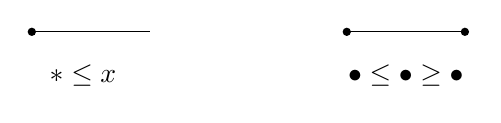
\begin{tikzpicture}
\draw (0,0) -- (1.5,0);
\fill (0,0) circle (1.5pt);
\node at (0.65,-0.55) {$\ast\leq x$};
\draw (4,0) -- (5.5,0);
\fill (4,0) circle (1.5pt);
\fill (5.5,0) circle (1.5pt);
\node at (4.75,-0.55) {$\bullet\leq\bullet\geq\bullet$};
\end{tikzpicture}
\end{adjustbox}
\end{center}

Комбинаторный пучок -- пучок, постоянный на каждом страте.

\underline{Гомологическая алгебра.}

$\mathcal A$ -- абелева категория (например, пучков над данным пр-вом или модулей)

$C(\mathcal A)$ -- категория комплексов над $\mathcal A$

надо знать \underline{производную категорию} (Verdier, 1961)

Объекты \Unclear{GELFAND-P001392}{objects-mark}{зачёркнутое «из»? / знак принадлежности?}
$C(\mathcal A)$
\begin{gather*}
\ldots\longrightarrow X^i\overset{d}{\longrightarrow}X^{i+1}
\overset{d}{\longrightarrow}X^{i+2}\longrightarrow\ldots\\
d^2=0
\end{gather*}
морфизмы -- морфизмы комплексов (наборы морф.
\begin{adjustbox}{max width=\linewidth}
\begin{tikzcd}[row sep=small]
X^i \arrow[d, "\varphi"'] \\
Y^i
\end{tikzcd}
\end{adjustbox}, перестан. с $d$)

$C(\mathcal A)$ -- тоже абелева категория

Огранич. комплексы (лишь конечное число $\neq0$) $C^b(\mathcal A)$

огранич. слева или справа $C^{\pm}(\mathcal A)$
\begin{gather*}
C^+(\mathcal A)\text{ -- огр. слева}\\
C^-(\mathcal A)\text{ -- огр. справа}
\end{gather*}

Гомотопическая категория $K(\mathcal A)$

объекты $K(\mathcal A)$ те же, что в $C(\mathcal A)$, а морфизмы -- классы эквив.
морфизмов $C(\mathcal A)$ относит. гомотопии.
\begin{equation*}
\operatorname{Hom}_{K(\mathcal A)}(X^\bullet,Y^\bullet)
\end{equation*}

Морфизм $X^\bullet\overset{\varphi}{\longrightarrow}Y^\bullet$ -- это [вставлено над строкой: такой]
набор $\varphi^i\colon X^i\longrightarrow Y^i$, что коммут. диаграмма:

[Слева:]
\begin{center}
\begin{adjustbox}{max width=\linewidth}
\begin{tikzcd}
X^{i-1} \arrow[r, "d"] \arrow[d, "{\varphi^{i-1}}"'] &
X^i \arrow[r, "d"] \arrow[d, "{\varphi^i}"] \arrow[dl, dashed, "{\psi^i}"'] &
X^{i+1} \arrow[d, "{\varphi^{i+1}}"] \arrow[dl, dashed, "{\psi^{i+1}}"'] \\
Y^{i-1} \arrow[r, "d"] & Y^i \arrow[r, "d"] & Y^{i+1}
\end{tikzcd}
\end{adjustbox}
\end{center}
[Справа:]
\begin{center}
\begin{adjustbox}{max width=\linewidth}
\begin{tikzcd}
X^i \arrow[r, "d"] \arrow[d, "{\varphi^i}"'] & X^{i+1} \arrow[d, "{\varphi^{i+1}}"] \\
Y^i \arrow[r, "d"] & Y^{i+1}
\end{tikzcd}
\end{adjustbox}
\end{center}
[Волнистая линия огибает левую диаграмму сверху и справа, затем проходит под правой.]

$\varphi$ нз. \underline{гомотопным нулю}, если $\exists$ набор отобр.
$X^i\overset{\psi^i}{\longrightarrow}Y^{i-1}$,
такой что
\begin{equation*}
\varphi^i=d\psi^i+\psi^{i+1}d\tag{1}
\end{equation*}

\SourcePage{GELFAND-P001393}{13}
\underline{Упражнение 1.}\quad Проверить, что для любой системы отобр. $\psi^i$ набор (1)
даёт морфизм комплексов, т.е. $d\varphi_i=\varphi_{i+1}d$.

\underline{Упражнение 2.}\quad Морфизмы, гомотопные $0$, образуют идеал, т.е. если
$\varphi$ гомотопен $0$ и $\varphi_1$ -- любой морфизм, то
$\varphi\circ\varphi_1$ -- гомотопен $0$.

(и то же самое верно для композиции $\varphi_2\circ\varphi$ с любым морфизмом $\varphi_2$)
\begin{equation*}
\operatorname{Hom}_{K(\mathcal A)}(X^\bullet,Y^\bullet)
=\operatorname{Hom}_{C(\mathcal A)}(X^\bullet,Y^\bullet)
/\bigl(\text{морфизмы, гомотопные }0\bigr)
\end{equation*}
Есть очевидные функторы
\begin{equation*}
\mathcal A\longrightarrow C(\mathcal A)\longrightarrow K(\mathcal A)
\end{equation*}
Функтор когомологий
\begin{equation*}
H^i\colon C(\mathcal A)\longrightarrow\mathcal A\qquad
\left(H^i(X^\bullet)=
\frac{\ker(d\colon X^i\longrightarrow X^{i+1})}
{\operatorname{Im}(d\colon X^{i-1}\longrightarrow X^i)}\right)
\end{equation*}

\underline{Упражнение 3.}\quad Док., что $\exists!$ функтор
$H^i\colon K(\mathcal A)\longrightarrow\mathcal A$, такой что
\begin{center}
\begin{adjustbox}{max width=\linewidth}
\begin{tikzcd}
C(\mathcal A) \arrow[r] \arrow[dr, "{H^i}"'] & K(\mathcal A) \arrow[d, "{H^i}"] \\
& \mathcal A
\end{tikzcd}
\end{adjustbox}
\end{center}
На морфизмах $H^i$ тоже очев. образом определяется.

\underline{Определение.}\quad $\varphi\colon X^\bullet\longrightarrow Y^\bullet$
[под стрелкой: в кат. $K(\mathcal A)$]
нз. \underline{квазиизоморфизмом}, если он индуц. изоморфизм
\begin{equation*}
H^i(X^\bullet)\longrightarrow H^i(Y^\bullet).
\end{equation*}

\underline{Производная категория.}

\underline{Упражнение 4.}\quad Пусть есть 3 комплекса
\begin{center}
\begin{adjustbox}{max width=\linewidth}
\begin{tikzcd}
X^\bullet & & Y^\bullet \\
& Z^\bullet \arrow[ul, "\alpha"] \arrow[ur, "\beta"'] &
\end{tikzcd}
\end{adjustbox}
\end{center}
и морфизмы, причём $\alpha$ -- квазиизоморфизм.

Тогда сущ. диаграмма (коммутативная)
\begin{center}
\begin{adjustbox}{max width=\linewidth}
\begin{tikzcd}
& Z' & \\
X^\bullet \arrow[ur, "{\alpha'}"] & & Y^\bullet \arrow[ul, "{\beta'}"'] \\
& Z^\bullet \arrow[ul, "\alpha"] \arrow[ur, "\beta"'] &
\end{tikzcd}
\end{adjustbox}
\end{center}
[Слева от нижней части диаграммы зачёркнуто:
\Unclear{GELFAND-P001393}{cancelled-left}{в к-рой?}.]

в к-рой $\beta'$ -- квазиизоморфизм.

То же справедливо, если начинать с диагр.
\begin{center}
\begin{adjustbox}{max width=\linewidth}
\begin{tikzcd}
& Z' & \\
X^\bullet \arrow[ur, "{\alpha'}"] & & Y^\bullet \arrow[ul, "{\beta'}"']
\end{tikzcd}
\end{adjustbox}
\end{center}
с квазиизоморфизмом $\alpha'$.

\SourcePage{GELFAND-P001394}{unlabelled}
\underline{Производная категория} $D(\mathcal A)$

Объекты $=$ объекты $K(\mathcal A)$ (т.е. комплексы)

Морфизмы [вставлено над строкой: $X^\bullet\longrightarrow Y^\bullet$] -- классы эквив. диаграмм
\begin{center}
\begin{adjustbox}{max width=\linewidth}
\begin{tikzcd}
X^\bullet & & Y^\bullet \\
& Z^\bullet \arrow[ul, "\alpha"] \arrow[ur, "\beta"'] &
\end{tikzcd}
\end{adjustbox}
\qquad $\beta\alpha^{-1}$
\end{center}
($\alpha$ -- квазиизоморфизм)

по отнош. эквивалентности, \underline{порожденному}
\Unclear{GELFAND-P001394}{elementary-abbrev}{элм.? / элем.?} отношением

[Зачёркнуто: \Unclear{GELFAND-P001394}{cancelled-there}{Есть? / Если?}.]

(Есть функтор $K(\mathcal A)\longrightarrow D(\mathcal A)$)

\begin{center}
\begin{adjustbox}{max width=\linewidth}
\begin{tikzcd}
X^\bullet & & Y^\bullet \\
& Z^\bullet \arrow[ul, "\alpha"] \arrow[ur, "\beta"'] & \\
& T \arrow[u, "\gamma"] &
\end{tikzcd}
\end{adjustbox}
\end{center}

\Unclear{GELFAND-P001394}{fraction-relation}{$\beta\alpha^{-1}\sim\beta\gamma(\alpha\gamma)^{-1}$?},
где $\gamma$ -- квазиизоморфизм.

\begin{center}
\begin{adjustbox}{max width=\linewidth}
\begin{tikzcd}
X^\bullet & & Y^\bullet \\
& Z^\bullet \arrow[ul, "\alpha"] \arrow[ur, "\beta"'] &
\end{tikzcd}
\end{adjustbox}
\quad $\sim$ \quad
\begin{adjustbox}{max width=\linewidth}
\begin{tikzcd}
X^\bullet & & Y^\bullet \\
& T \arrow[ul, "{\alpha\gamma}"] \arrow[ur, "{\beta\gamma}"'] &
\end{tikzcd}
\end{adjustbox}
\end{center}

Теперь эти морфизмы можно компоновать.

\begin{center}
\begin{adjustbox}{max width=\linewidth}
\begin{tikzcd}
X^\bullet & & Y^\bullet & & W \\
& Z^\bullet \arrow[ul] \arrow[ur] & & T \arrow[ul] \arrow[ur] & \\
& & S \arrow[ul] \arrow[ur] & &
\end{tikzcd}
\end{adjustbox}
\end{center}
[Справа от нижней части диаграммы стрелка влево с подписью:]
$\longleftarrow$ достраиваем \underline{по лемме}

композиция -- внешняя сторона диаграммы


\SourcePage{GELFAND-P001395}{unlabelled}
\underline{19.10.87.}\quad \underline{Сем. Гельфанда.}

\underline{И.М. Гельфанд}\quad
\underline{Вычисление сумм $k$-х степеней и прочих сумм}

\Unclear{GELFAND-P001395}{speaker-parenthesis}{(по недавней мысли) / (по неясной мысли)}

\begin{equation*}
F'(x)=f(x)\qquad f(x)=x^k;\qquad F(x)=\frac{x^{k+1}}{k+1}
\end{equation*}
\begin{align*}
F(2)-F(1)&=\frac{f(1)}{1!}+\frac{f'(1)}{2!}+\frac{f''(1)}{3!}+\ldots\\
F(3)-F(2)&=\frac{f(2)}{1!}+\frac{f'(2)}{2!}+\frac{f''(2)}{3!}+\ldots\\[8pt]
F(n+1)-F(n)&=f(n)+\frac{f'(n)}{2!}+\frac{f''(n)}{3!}+\ldots
\end{align*}
\rule{9cm}{0.3pt}
\begin{equation*}
F(n+1)-F(1)=S_0+\frac{S_1}{2!}+\frac{S_2}{3!}+\ldots
\end{equation*}
аналогично,
\begin{align*}
f(n+1)-f(1)&=S_1+\frac{S_2}{2!}+\ldots\\
f'(n+1)-f'(1)&=S_2+\frac{S_3}{2!}+\ldots\\
\ldots\qquad&\ldots\\
f^{(p)}(n+1)-f^{(p)}(1)&=\ldots\quad
\Unclear{GELFAND-P001395}{system-last-index}{S_p}+\ldots
\end{align*}

[Справа от системы:]
Здесь
\begin{align*}
S_0&=f(1)+f(2)+\ldots+f(n)\\
S_1&=f'(1)+f'(2)+\ldots+f'(n)\\
&\ldots\\
S_k&=f^{(k)}(1)+f^{(k)}(2)+\ldots+f^{(k)}(n)
\end{align*}

Отсюда
[слева от определителя зачеркнуто:
\Unclear{GELFAND-P001395}{determinant-cancellation}{det / неразборчиво}]
\begin{equation*}
S_0=\frac{
\begin{vmatrix}
F(n+1)-F(1)&\dfrac{1}{2!}&\dfrac{1}{3!}&\ldots\\
f(n+1)-f(1)&1&\dfrac{1}{2!}&\\
f'(n+1)-f'(1)&0&1&\\
\ldots&0&0&
\end{vmatrix}}{1}
\end{equation*}

Разложим по 1-му столбцу
\begin{equation*}
S_0=A_0\bigl(F(n+1)-F(1)\bigr)
+A_1\bigl(f(n+1)-f(1)\bigr)+\ldots
\end{equation*}
коэфф. универ. — годится для $\forall$ ф-и!!

Подставим $f(x)=e^{tx}$

возникают ленточные детерминанты!

[Зачеркнуто:
\Unclear{GELFAND-P001395}{exponential-cancellation}{$S_0=A_0$ / неразборчиво}]
\begin{equation*}
\Unclear{GELFAND-P001395}{exponential-fraction}{\frac{\dfrac{1}{n+1}e^{t(n+1)}-e}{e^t-1}}
\end{equation*}
разложим [зачеркнуто:
\Unclear{GELFAND-P001395}{series-cancellation}{ряд / неразборчиво}]
по $t$\quad $\Longrightarrow$ \underline{числа Бернулли}

\underline{Задача.} Симм. группа $S_n$
\Unclear{GELFAND-P001395}{symmetric-group-predicate}{порождается / определяется}
[вставлено над строкой: «(\Unclear{GELFAND-P001395}{group-generator-abbreviation}{обрц. / обр.} $s_1,\ldots,s_{n-1}$)»]
соотношениями
\begin{equation*}
s_i^2=1,\qquad s_i s_j=s_j s_i\quad\text{при }|i-j|\ge2,
\qquad (s_i s_{i+1})^3=1
\end{equation*}
Рассм. парабол.- подгруппу
\begin{equation*}
G=\Sigma_n,\qquad H=\Sigma_k\times\Sigma_{n-k},\qquad G\supset H
\end{equation*}
\begin{equation*}
\mathcal A=\mathbb C[G]=
\left\{\sum_{g\in G}a_g g,\quad a_g\in\mathbb C\right\}
\end{equation*}

\SourcePage{GELFAND-P001396}{23}
\begin{equation*}
\mathcal A\supset
\underset{\text{подалгебра}}{\mathcal A'}
=\{x\in A,\ xh=hx=x\text{ для любых }h\in H\}
\end{equation*}

[Зачеркнутый знак перед заголовком:
\Unclear{GELFAND-P001396}{heading-cancellation}{неразборчиво}]
\underline{Бейлинсон А.}\quad (продолжение)

\underline{Производные категории}

\begin{adjustbox}{max width=\linewidth}
\begin{tikzcd}[row sep=small,column sep=small]
\mathcal A\arrow[d]&\text{— абелева категория}\\
C(\mathcal A)\arrow[d]&\text{— кат. комплексов над }\mathcal A\\
K(\mathcal A)\arrow[d]&\text{— гомотопич. категория}\\
D(\mathcal A)&\text{— производная категория}
\end{tikzcd}
\end{adjustbox}

объекты $D(\mathcal A)$ — комплексы, а морфизмы — классы эквив. диаграмм

\SourceFigure{GELFAND-P001396}{roof-cancellation}{Зачеркнутая диаграмма: $X$ слева вверху, $Y$ справа вверху, $Z$ ниже между ними; видны наклонные штрихи от нижнего узла к верхним и широкая многократная зигзагообразная отмена. Точные черты стрелок под зачеркиванием не устанавливаются.}

\begin{adjustbox}{max width=\linewidth}
\begin{tikzcd}[row sep=small,column sep=small]
&Z'&\\
X\arrow[ur]&&Y\arrow[ul,shorten <=8pt,shorten >=8pt]\\
&Z\arrow[ul,shorten <=8pt,shorten >=8pt]\arrow[ur]&
\end{tikzcd}
\end{adjustbox}
\quad (квазиизоморфизмы короче).

\underline{Пример 1.} Пусть $X$ — комплекс с
[зачеркнуто: \Unclear{GELFAND-P001396}{example-cancellation}{со / неразборчиво}]
$H^i(X)=0$ при $i\ne0$.
Тогда $X$ канонически квазиизоморфен $H^0(X)$:
\begin{equation*}
X\cong H^0(X)\text{ в }D(\mathcal A)
\end{equation*}
(В гомотопической категории это не так!)

Для комплекса $X$ введем подкомплекс $\tau_{\le0}(X)$ в $X$:
\begin{equation*}
\text{(1)}\qquad
\tau_{\le0}(X)^i=
\begin{cases}
X^i,&i<0\\
\ker d:X^0\to X^1,&i=0\\
0,&i>0
\end{cases}
\end{equation*}
Легко видеть, что
\begin{equation*}
\text{(2)}\qquad
H^j(\tau_{\le0}(X))=
\begin{cases}
H^j(X),&j\le0\\
0,&j>0
\end{cases}
\end{equation*}
Диаграмма

(3)
\SourceFigure{GELFAND-P001396}{truncation-diagram}{Снизу расположен $\tau_{\le0}(X)$; от него идут стрелки вверх-влево к $X$ и вверх-вправо к $H^0(X)$. У правой стрелки стоит $\sim$. У левой стрелки знак, похожий на повернутую тильду, $2$ или $\iota$; ниже слева подпись «кан. вкл.». Справа от диаграммы отдельный короткий крючкообразный штрих.}

задаёт искомый изоморфизм в $D(\mathcal A)$.

[Зачеркнуто:
\Unclear{GELFAND-P001396}{cancelled-bottom-sentence}{Этот же комплекс можно было смотреть на}]

\underline{Замечание.} комплекс $X$ с несколькими отл. от $0$ группами $H^i$
\underline{не} квазиизоморфен (вообще говоря) сумме, а если
[вставлено над строкой: «(квази)»] есть, то неединственным образом.

\SourcePage{GELFAND-P001397}{unlabelled}
\underline{Структура триангулированной категории}

$K(A)$ и $D(A)$ не явл. абелевыми категориями.

\underline{Упражнение 1.} Проверить, что
$K(A)$ — абелева $\Longleftrightarrow\mathcal A$ полупроста

($\mathcal A$ — полупроста $\Longleftrightarrow$
$[(\forall\text{ объект})=(\text{прямая сумма неприводимых})]$).

\underline{Конус морфизма.}

Пусть $f:X\longrightarrow Y$\quad морфизм комплексов

\begin{adjustbox}{max width=\linewidth}
\begin{tikzcd}[row sep=small,column sep=large]
X^1\arrow[r,"f^1"]\arrow[dr,dashed,no head]&Y^1\\
X^0\arrow[u]\arrow[r,"f^0"]\arrow[dr,dashed,no head]&Y^0\arrow[u]\\
X^{-1}\arrow[u]\arrow[r,"f^{-1}"]&Y^{-1}\arrow[u]
\end{tikzcd}
\end{adjustbox}

рассм. это всё как бикомплекс, т.е.
напишем комплекс
\begin{equation*}
C(f)^i=\Unclear{GELFAND-P001397}{cone-coordinate-order}{Y^i\oplus X^{i+1}}
\end{equation*}
\begin{equation*}
d(x,y)=(-d(x),d(y)+f(x))
\end{equation*}

Имеется последовательность
\begin{equation*}
\text{(4)}\qquad
C(f[-1])\longrightarrow X\overset{f}{\longrightarrow}Y
\underset{g}{\longrightarrow}C(f)\longrightarrow X[1]\longrightarrow
\end{equation*}
[Над стрелкой $Y\to C(f)$ зачеркнуто:
\Unclear{GELFAND-P001397}{sequence-arrow-cancellation}{неразборчиво};
под $g$: «вкл.».]
[Перед $C(f)$ зачеркнуто:
\Unclear{GELFAND-P001397}{sequence-object-cancellation}{$X$ / $Y$}.]
[Под $X[1]$: «сдвиг градуировки и изменён знак $d$».]
\begin{equation*}
\longrightarrow Y(1)\longrightarrow
\Unclear{GELFAND-P001397}{sequence-shifted-cone}{C(f[1])\text{ / }C(f)[1]}
\longrightarrow X[2]\longrightarrow
\end{equation*}
[Между $X$ и $[2]$ зачеркнуто:
\Unclear{GELFAND-P001397}{sequence-shift-cancellation}{( / [1] / неразборчиво}.]

она перех. в себя при сдвиге на 3 шага.
В гомотопич. категории она перех. в себя при сдвиге на шаг.

\begin{equation*}
\text{(5)}\qquad Y\overset{g}{\longrightarrow}C(f)\longrightarrow C(g)
\end{equation*}
(6) \underline{Утвержд.} В $K(A)$ комплекс $C(g)=X[1]$.

Имеется отображение:
\begin{adjustbox}{max width=\linewidth}
\begin{tikzcd}[row sep=small,column sep=large]
Y\arrow[r]\arrow[d,equal]&C(f)\arrow[r]\arrow[d,equal]&X[1]\\
Y\arrow[r]&C(f)\arrow[r]&C(g)\arrow[u]
\end{tikzcd}
\end{adjustbox}

А именно,
\begin{equation*}
C(g)^i=C(f)^i\oplus Y^{i+1}=X^{i+1}\oplus Y^i\oplus Y^{i+1}
\end{equation*}
проектируется на $X^{i+1}$

\SourcePage{GELFAND-P001398}{24}
\underline{Упражнение 2}. Проверить, что это морфизм комплексов и
изоморфизм в гомотопической категории.

\underline{Упражнение 3}. Найти в $K(A)$ конусы $C(id)$ и $C(0)$
[Под $id$: тож. отобр.; под $0$: нулевое отобр.]

\underline{Определение 1}. Треугольником в $K(A)$ или $D(A)$ называется
диаграмма
\begin{center}
\begin{adjustbox}{max width=\linewidth}
\begin{tikzcd}[column sep=small]
\cdots \arrow[r] & Z[-1] \arrow[r,"{\gamma[-1]}"] & X \arrow[r,"\alpha"] &
Y \arrow[r,"\beta"] & Z \arrow[r,"\gamma"] & X[1] \arrow[r,"{\alpha[1]}"] &
Y[1] \arrow[r,"{\beta[1]}"] & Z[1] \arrow[r,"{\gamma[1]}"] & \cdots
\end{tikzcd}
\end{adjustbox}
\end{center}

[Зачёркнуто: \SourceFigure{GELFAND-P001398}{cancelled-sketch}{Набросок под диаграммой: слева почти вертикальный штрих с направленным вверх концом, справа наклонный штрих с направленным вверх вправо концом; между ними и поверх них несколько наклонных линий зачёркивания. Возможные буквенные подписи под зачёркиванием не различаются уверенно.}]

\underline{\underline{Опред. 2}}. Точным треугольником в $K(A)$ или $D(A)$ наз.
треугольник, изоморфный треугольнику:
\begin{center}
\begin{adjustbox}{max width=\linewidth}
\begin{tikzcd}[column sep=small]
{} \arrow[r] & X \arrow[r,"f"] & Y \arrow[r,"g"] & C(f) \arrow[r] &
X[1] \arrow[r] & Y[1] \arrow[r] & \cdots
\end{tikzcd}
\end{adjustbox}
\end{center}

\SourcePage{GELFAND-P001399}{unlabelled}
\underline{9/XI-87 г.}\qquad \underline{\underline{Сем. Гельфанда}}

[Зачёркнуто: Ласку.]\qquad \underline{Ласку}

\underline{И.М.Г. по мотивам Ласку}
(\Unclear{GELFAND-P001399}{heading-parenthesis}{красивые / правильные} ряды)

Полиномы Шуберта.

Рассм. многочлен
\begin{equation*}
P=\alpha u+\beta\Unclear{GELFAND-P001399}{equation-1-second-variable}{u\text{ или }v}+\gamma w+\cdots \tag{1}
\end{equation*}
$u,v,w$ [зачёркнуто: \Unclear{GELFAND-P001399}{cancelled-coefficients}{$\alpha,\beta,\gamma$}] — одночлены

В нашем случае будет $u,v,w,$ [зачёркнут один знак:
\Unclear{GELFAND-P001399}{cancelled-after-w}{неразборчиво}] $\ldots=x_1,x_2,\ldots,x_n$

$\alpha,\beta,\gamma,\ldots$ — числа

Многочлены [зачёркнуто: \Unclear{GELFAND-P001399}{cancelled-before-sm}{ф-я / ф-и}]
$S^m(P)$ [зачёркнуто: \Unclear{GELFAND-P001399}{cancelled-after-sm}{Шура}]
определяются по ф-ле
\begin{equation*}
\sum_{\Unclear{GELFAND-P001399}{equation-2-lower-bound}{m\ge0\text{ или }m=0}}^{\infty}
z^m S^m(P)=\frac{1}{(1-zu)^\alpha(1-zv)^\beta\ldots} \tag{2}
\end{equation*}
\begin{equation*}
\alpha=\beta=\gamma=\cdots=1\quad\Rightarrow
\end{equation*}
\begin{equation*}
S^m(x_1+x_2+\cdots+x_n)=\sum_{i_1\le i_2\le\cdots\le i_m}
x_{i_1}x_{i_2}\cdots x_{i_m} \tag{3}
\end{equation*}

Например,
\begin{equation*}
S^2(x_1+x_2)=x_1^2+x_1x_2+x_2^2
\end{equation*}

Рассмотрим ганкелеву матрицу (бес. порядка)
\begin{equation*}
\begin{pmatrix}
S^0(P)&S^1(P)&S^2(P)&\ldots\\
S^{-1}(P)&S^0(P)&S^{\Unclear{GELFAND-P001399}{matrix-row-2-col-3}{4\text{ или }1}}(P)&\ldots\\
&&&
\end{pmatrix},\qquad S^{-i}(P)=0\text{ при }i>0. \tag{4}
\end{equation*}

(см. кн. \underline{Ахиезера} о пробл. моментов)

Умножению рядов (2) соответствует умножение матриц (4).

\SourcePage{GELFAND-P001400}{30}
\underline{Тема по теории операторов, к-рую И.М.Г. предложил
\Unclear{GELFAND-P001400}{heading-recipient}{Бирману / Бурману}:}

\Unclear{GELFAND-P001400}{heading-verb}{Связать / Связь / Сделать}
$K$-функтор в теории операторов

(на 15 лет позже уже это сделал Сато)

и это стало модой.

\underline{Единств. теорема из теории матриц}

Рассм. матрицу $A$: $f_{\alpha\beta}=f(\alpha,\beta)$ и все её миноры
$k$-го порядка: это тоже матрица (присоед. матр. $k$-го порядка)
$\Lambda^k(A)$. Тогда
\begin{equation*}
\Lambda^k(AB)=\Lambda^k(A)\Lambda^k(B) \tag{5}
\end{equation*}

Номера строк выгодно обозначать $i_1+1,i_2+2,\ldots,i_p+p$, а столбцов
$j_1+1,j_2+2,\ldots,j_p+p$
\begin{equation*}
\left|\begin{aligned}
i_1&\le i_2\le\cdots\le i_p\\
j_1&\le\cdots\le j_p
\end{aligned}\right.
\end{equation*}

\begin{equation*}
S_{J\mid I}(P)\quad\text{— соотв. минор, наз. }\underline{\text{косая функция Шура}}. \tag{6}
\end{equation*}
\begin{equation*}
S_{J\mid 0}(P)\quad\text{— обычная ф-я Шура.}
\end{equation*}

[Зачёркнуто: Тогда] Можно рассм. многочлен (Якоби)
\begin{equation*}
\frac{
\begin{vmatrix}
x_1^{j_1}&x_1^{j_2+1}&\ldots&x_1^{j_p+p-1}\\
x_2^{j_1}&x_2^{j_2+1}&\ldots&x_2^{j_p+p-1}\\
\ldots&\ldots&\ldots&\ldots
\end{vmatrix}
}{
\begin{vmatrix}
1&x_1&\ldots&x_1^{p-1}\\
1&x_2&\ldots&x_2^{p-1}\\
&&&\\
1&x_p&\ldots&x_p^{p-1}
\end{vmatrix}
} \tag{7}
\end{equation*}
[В первых двух строках числителя после $j_1$ зачёркнуто:
\Unclear{GELFAND-P001400}{numerator-first-column-cancellations}{$+1$ / $+0$}.]

[Справа от числителя: \Unclear{GELFAND-P001400}{right-of-numerator}{1 / одиночный косой штрих}.]

(\Unclear{GELFAND-P001400}{exercise-number}{8 / 7})
([Вписано над строкой: \underline{Упр}] проверить, что числитель делится на знаменатель!)

[Зачёркнуто: \Unclear{GELFAND-P001400}{cancelled-before-eto}{ко / но}.]
Это симметрич. ф-я, но коэффициенты явно не
[зачёркнуто: \Incomplete{GELFAND-P001400}{cancelled-right-word}{Зачёркнутое слово под вставленным «пишутся» не прочитано.}]
[вписано над строкой: \underline{пишутся}]
и до сих пор исследуются

[На левом поле: (\Unclear{GELFAND-P001400}{margin-first-line}{первые шаги / новые шаги}
\Incomplete{GELFAND-P001400}{margin-second-line}{Вторая строка мелкой приписки перед библиографической ссылкой не прочитана.})]

(см. раб. [зачёркнутые инициалы:
\Unclear{GELFAND-P001400}{bibliography-cancelled-initials}{И.Г. / И.М.};
над ними вписано: \underline{И.М.}] Гельфанд, Зелевинский, 1986, ФА;
и непечатная раб. Б. \Unclear{GELFAND-P001400}{bibliography-last-name}{Лидского / Литского})

\underline{Ясно} \Unclear{GELFAND-P001400}{penultimate-word}{пока / лишь}, что коэффициенты
[зачёркнуто: \Unclear{GELFAND-P001400}{cancelled-before-integers}{все / будут}] целые.

Шур понял, что они важны:
\Unclear{GELFAND-P001400}{last-line-verb}{прокомментировал / прокомментировав}
Якоби, Фробениуса и др.

\SourcePage{GELFAND-P001401}{unlabelled}

Фробениус нашёл характеры симм. группы; это глубокая работа, которую
не заменяют комментарии Г. Вейля.

(9) \underline{Теорема.} (Якоби -- Труди)

\begin{equation*}
(10)\qquad (7)=S_{J/0}(x_1+\ldots+x_p)
\end{equation*}

(11) \underline{Задача:} а) \Unclear{GELFAND-P001401}{task-a}{осадить / осознать};

б) дать её классич. док-во;

в) дать интерпрет. в теории представлений.

(12) $S_{J/I}$ удовл. системе тождеств;
это плюккеровы координаты (одно из достиж. Сато!)

\begin{equation*}
(13)\qquad
S^{\text{\Unclear{GELFAND-P001401}{formula-13-power}{n / m}}}(P+Q)
=\sum_j S^{n-j}(P)S^j(Q);
\end{equation*}

\begin{equation*}
(14)\qquad
S^n(PQ)=\sum_{|J|=n}S_J(P)S_J(Q),\qquad S_J=S_{J/0};
\end{equation*}

\begin{equation*}
(15)\qquad
S^n(S^m(P))=\sum(n,m;J)S_J(P)
\quad\text{\Unclear{GELFAND-P001401}{formula-15-end}{$\Vert$ / зачёркнутый знак}},
\end{equation*}

где $(n,m;J)$ --- универс. коэффициенты.

Когомол. флаговых мн-зий счит. 2-мя способами

а) разб. на клетки Шуберта (размерности чётны!)

б) дифф. формы;

какие формы соответ. каким клеткам?

Там возник. полиномы Шуберта

(с точн. до симметрических)

\underline{Ласку, Шютценберже:} надо забыть о топологии и считать полиномы.

Полиномы надо \Unclear{GELFAND-P001401}{last-line-word}{поселить} в кольце всех мног. и т. д.

\SourcePage{GELFAND-P001402}{31}

[Следующий фрагмент обведён и зачёркнут:]

(16) \underline{Теорема.} Переставим строки
\begin{equation*}
h_1+1,\ h_2+2,\ldots,h_p+p,\qquad h_1\le h_2\le\ldots\le h_p;
\end{equation*}

Ньютон ввёл операции

\begin{equation*}
(16)\qquad
\partial_i f(x_1,\ldots,x_n)=
\frac{f(x_1,\ldots,x_{i+1},x_i,\ldots,x_n)-f(x_1,\ldots,x_i,x_{i+1},\ldots,x_n)}{x_{i+1}-x_i}
\end{equation*}

Тогда

\begin{equation*}
(17)\qquad
\left\{
\begin{aligned}
&\partial_i^2=0\\
&\partial_i\partial_j=\partial_j\partial_i,\qquad |i-j|\ge2,\\
&\partial_i\partial_{i+1}\partial_i=\partial_{i+1}\partial_i\partial_{i+1}
\end{aligned}
\right.
\end{equation*}

(18) \underline{Замечание.}
\begin{equation*}
(\partial_i+1)(\partial_i-q)=0
\quad\Rightarrow\quad
\partial_i\text{ --- $q$-аналог образующих симм. группы}
\end{equation*}
\begin{equation*}
q=1\quad\Rightarrow\quad\text{симм. группа}
\end{equation*}

(вместо $(17)_{\text{\Unclear{GELFAND-P001402}{remark-18-subscript}{1 / a}}}$)

\underline{\underline{Ласку}}

\underline{Связь многочленов Шуберта с ф-ями Шура.}

(19) $\partial_i(fg)=g\partial_i(f)$, если
[зачёркнуто: \Unclear{GELFAND-P001402}{cancelled-19-symbol}{$f$}]
$g$ симметрична отн.
[зачёркнуто: \Incomplete{GELFAND-P001402}{cancelled-19-word}{Слово закрыто несколькими штрихами; возможны «всех» / «двух», чтение целого слова не установлено.}]
перем. $x_i,x_{i+1}$.

Напоминание о пол. Шуберта
\begin{equation*}
Y_{730}=x_1^7x_2^3x_3^0
\end{equation*}

(20) \underline{Опр.} Если $\underbrace{i_1\ge i_2\ge i_3\ge\ldots}_{I}$, то
$x_1^{i_1}x_2^{i_2}\ldots=Y_I$

(мног. Шуберта
[зачёркнуто: \Unclear{GELFAND-P001402}{note-20-first-sign}{$I$ / $=$}]
[зачёркнуто: \Incomplete{GELFAND-P001402}{note-20-cancelled-word}{Короткая запись закрыта горизонтальными штрихами; целые буквы и слово не восстанавливаются по скану.}]
с индексом $I$ одночлен)

Все мн. Шуберта \Unclear{GELFAND-P001402}{all-schubert-sign}{$=$}
образы этих под. дейст. произвольной сов. $\partial_i$.

[Над словом «образы» вписано: «(все ненулевые)».]

\underline{Правило \Unclear{GELFAND-P001402}{rule-abbreviation}{расч. / раб.} индексов}

\begin{equation*}
(21)\qquad
Y_{\ldots i_p i_{p+1}\ldots}
\overset{\partial_p}{\longrightarrow}
\begin{cases}
Y_{\ldots i_{p+1}\,i_p-1},&i_p>i_{p+1}\\
0,&\text{otherwise}
\end{cases}
\end{equation*}

\underline{Упр.:} Док. корректность этих определений.

(22) \underline{Пример}
\begin{equation*}
Y_{730}=x_1^7x_2^3x_3^0=
\begin{vmatrix}
S^3(x_1+x_2)&S^8(x_1)\\
S^2(x_1+x_2)&S^7(x_1)
\end{vmatrix}
\end{equation*}

\SourcePage{GELFAND-P001403}{unlabelled}

(23)

[В первой строке после дроби, перед знаком равенства, зачёркнуто:
\Incomplete{GELFAND-P001403}{generating-cancelled}{Короткая запись пересечена горизонтальной чертой; видимые нижние дуги и правый штрих не позволяют установить текст или формулу.}]

\begin{equation*}
\begin{adjustbox}{max width=\linewidth}
\begin{tikzcd}[column sep=small,row sep=large]
{\displaystyle\frac{1}{(1-zx_1)(1-zx_2)}}\arrow[d,"\partial_2"]
& {=\displaystyle\sum z^j S^j(x_1+x_2)}\\
{\displaystyle\frac{z}{(1-zx_1)(1-zx_2)(1-zx_3)}} &
\end{tikzcd}
\end{adjustbox}
\end{equation*}

\begin{equation*}
(23)\qquad
S^n(x_1+x_2)\overset{\partial_2}{\longrightarrow}
S^{n-1}(x_1+x_2+x_3)
\end{equation*}

Из (22) получим

(24)
\begin{equation*}
\begin{adjustbox}{max width=\linewidth}
\begin{tikzcd}[column sep=small,row sep=large]
{\partial_2Y_{730}}
& {=\begin{vmatrix}S^2(x_1+x_2+x_3)&S^8(x_1)\\S^1(x_1+x_2+x_3)&S^7(x_1)\end{vmatrix}}
& {=Y_{702}}\arrow[d,"\partial_1"]\\
& {\begin{vmatrix}S^2(x_1+x_2+x_3)&S^7(x_1+x_2)\\S^1(x_1+x_2+x_3)&S^6(x_1+x_2)\end{vmatrix}}\arrow[d,"\partial_2"]
& {=Y_{062}}\\
{Y_{025}}\arrow[d,equal]
& {=\begin{vmatrix}S^2(x_1+x_2+x_3)&S^6(x_1+x_2+x_3)\\S^1(x_1+x_2+x_3)&S^5(x_1+x_2+x_3)\end{vmatrix}}
&\\
{S_{025}(x_1+x_2+x_3)}&&
\end{tikzcd}
\end{adjustbox}
\end{equation*}

(ф-я Шура, опред. ранее; $S_{025/0}(x_1+x_2+x_3)$,
наборы нулей опускаются)

Запись формулы
[зачёркнуто: \Incomplete{GELFAND-P001403}{bottom-cancelled-word}{Слово покрыто несколькими пересекающимися штрихами; предположение «Шура» не подтверждается целиком видимыми буквами.}]
(22) в виде дет. использовалась
в теории исключения в 19 веке.

\underline{Есть 5 томов (толстых) книги}

\underline{T. Muir}: History of Determinants, Dover (1960)

\SourcePage{GELFAND-P001404}{32}

Ещё есть книга (его же)

Theory of determinants

(\Unclear{GELFAND-P001404}{book-parenthesis}{только ф-лы / тысячи ф-л})

(1 том)

\underline{500 страниц}

[Справа от заглавия, две записи, разделённые вертикальной чертой:]
всё до \fbox{1900} $\vert$ почти всё до (1920)

[Стрелка вниз от названия книги:] есть в ИПМ.

\underline{Аналогия}: теория интегрир. систем, \Unclear{GELFAND-P001404}{analogy-verb}{соорудить / содержит / сооружать} теорию под эти ф-лы.

(25) \underline{Теорема.}
\Unclear{GELFAND-P001404}{theorem25-left-index}{$S_{I\mid000}$ / $S_{I1000}$}
$(x_1+\dots+x_n)=Y_{i_1\dots i_n0000}$

$0\leq i_1\leq\dots\leq i_n$

(26) Finite case:
\Unclear{GELFAND-P001404}{finite26-left}{$\mathbb{Z}[x_1,x_2,\dots,x_n]$ / $\mathbb{Z}[x_1,x_2,\dots,x_{n+1}]$}
$\big/$ideal of symm. pol. in
$(x_1,x_2,$
[зачёркнуто: \Unclear{GELFAND-P001404}{finite26-cancelled}{$x_3$? / $x_n$?}]
$\dots,x_{n+1})$

(27) \underline{Теорема.} Полиномы Шуберта

(28)
\begin{equation*}
Y_I,\quad 0\leq i_1\leq n,\quad
0\leq i_2\leq n-1,\quad\dots,\quad
0\leq i_{n+1}\leq0
\end{equation*}
образуют базис в кольце (26) как в своб. абелевой группе.

\underline{Пример}

$\underline{n=2}\qquad\mathfrak{S}(3);$
\begin{equation*}
Y_{210}\qquad Y_{110}\qquad Y_{200}\qquad
Y_{010}\qquad Y_{100}\qquad Y_{000}
\end{equation*}
$\mathbb{Z}$-базис в $\mathbb{Z}[x_1,x_2,x_3]/(\qquad)$

Из (27) видно, что размерность есть
\Unclear{GELFAND-P001404}{dimension-factorial}{$n!$ [так в источнике]}.

Остальные попадают в идеал:

(29)
\begin{equation*}
Y_I\in\mathrm{ideal}\qquad\text{if}\qquad I\leq\!\!\!/\,210
\end{equation*}

(30) \underline{Вопрос И.М.Г.}: как пишется представление $\mathfrak{S}(n)$
[зачёркнуто: \Unclear{GELFAND-P001404}{question30-cancelled}{в? / неразборчивый знак}]
при действии $\mathfrak{S}(n)$ на переменные $x_1,\dots,x_n$ в многочленах
Шуберта

В кольце когомологий
[вставлено над строкой со знаком вставки:
(\Unclear{GELFAND-P001404}{cohomology-insertion}{мн-ия / мн-гия} флагов)]
есть квадр. форма, к-рая пишется так:

(31)
\begin{equation*}
PQ\overset{\partial_1\partial_2\partial_1}{\longrightarrow}(P,Q)
\end{equation*}
(скаляр. произведение)

[Справа:] (число в факторе по идеалу)

(32) \underline{Chevalley theorem.}

$\partial_1$ симметричен по отн. к $(\ ,\ )$

$\partial_2$ — '' — [знак повтора]

[Слева:] с.у.

(33)
\begin{equation*}
(\partial_1(P),Q)=(P,\partial_1(Q))
\end{equation*}

Док-во несложно.

Ласку.

(34)
\begin{equation*}
Y_I,\qquad Y_{I'},\qquad I+I'=n\quad n-1\quad\dots\quad1\quad0
\end{equation*}


\SourcePage{GELFAND-P001405}{unlabelled}
Тогда
\begin{equation*}
(Y_I,Y_J)=\text{\Unclear{GELFAND-P001405}{pairing-value}{0 или C}}
\quad\text{при }J\ne I'.\tag{35}
\end{equation*}
(всё в факторах)

\underline{Теорема:}

(36) $Z[x_1,x_2,x_3]$ — своб. модуль [вставлено над строкой: над]
$\underline{\operatorname{Sym}}(x_1,x_2,x_3)$
с базисом — полин. Шуберта.

Не все полин. Шуберта явл. детерминантами и поэтому вместо
них используются разд. разности $\partial_i$.

\underline{Зад. И.М.Г.} Обобщить теор. о характерах: непр. предст., характеры
\Unclear{GELFAND-P001405}{characters-line-ending}{с-…-}
-ф-и Шуберта.

\underline{След. раз будет Тахтаджян о квантовых группах.}

\underline{\underline{Капранов (Миша)}}

\underline{2-категории.}

Это алг. структ. с объектами 4-х типов
\begin{description}
\item[а)] объекты $\bullet$
\item[б)] гориз. морф. $\bullet\longrightarrow\bullet$
\item[в)] верт. морф. $\uparrow$
\item[г)] квадраты
\begin{adjustbox}{max width=\linewidth}
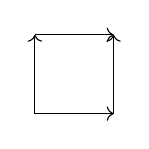
\begin{tikzpicture}[baseline=0.3cm]
\draw[->] (0,0)--(1,0);
\draw[->] (0,1)--(1,1);
\draw[->] (0,0)--(0,1);
\draw[->] (1,0)--(1,1);
\end{tikzpicture}
\end{adjustbox}
\end{description}

[На правом поле:]
Здесь $\begin{matrix}\longrightarrow\\\longrightarrow\end{matrix}$ гориз. морф.,
$\uparrow\ \uparrow$ верт. морф.
(их нач. и концы — 1-морфизмы).

Можно компонировать:
\begin{description}
\item[1)] $\longrightarrow\ \longrightarrow$ 2 гориз. морф.
\item[2)] $\begin{matrix}\uparrow\\\uparrow\end{matrix}$ 2 верт. морф.
\item[3)] квадр. двумя способами умножаются
\end{description}
\begin{center}
\begin{adjustbox}{max width=\linewidth}
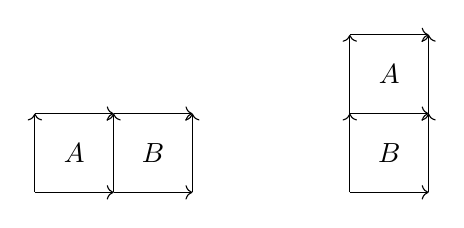
\begin{tikzpicture}
\draw[->] (0,0)--(1,0);
\draw[->] (1,0)--(2,0);
\draw[->] (0,1)--(1,1);
\draw[->] (1,1)--(2,1);
\draw[->] (0,0)--(0,1);
\draw[->] (1,0)--(1,1);
\draw[->] (2,0)--(2,1);
\node at (0.5,0.5) {$A$};
\node at (1.5,0.5) {$B$};
\draw[->] (4,0)--(5,0);
\draw[->] (4,1)--(5,1);
\draw[->] (4,2)--(5,2);
\draw[->] (4,0)--(4,1);
\draw[->] (4,1)--(4,2);
\draw[->] (5,0)--(5,1);
\draw[->] (5,1)--(5,2);
\node at (4.5,1.5) {$A$};
\node at (4.5,0.5) {$B$};
\end{tikzpicture}
\end{adjustbox}
\end{center}
(см. книгу Габриэля)
% Review coordinates (original pixels): pairing [720,125,890,280];
% characters ending [1980,1020,2360,1120]; full-page 2408 x 3448.

\SourcePage{GELFAND-P001406}{33}
\underline{Осн. нетрив. аксиома}: 2-мерн. ассоциативность

(1)
\SourceFigure{GELFAND-P001406}{interchange-diagram}{Слева два вертикальных прямоугольника: в первом $A$ над $B$, во втором $C$ над густо обведённым знаком, похожим на $D$; в каждом средняя горизонтальная стрелка направлена вправо. Между прямоугольниками кружок композиции, далее знак равенства. Справа верхний ряд содержит $A$, $C$, нижний — $B$, знак, похожий на $D$; между рядами узкая полоса с кружком. У концов полосы видны стрелочные и повторно обведённые штрихи, точное соединение которых неясно.}

\underline{Пример, когда не вып.}
[зачёркнуто: \Unclear{GELFAND-P001406}{example-cancel-left}{неразборчиво}]
акс.
[зачёркнуто: \Unclear{GELFAND-P001406}{example-cancel-right}{неразборчиво}]
(1)

\underline{Тензоры:}
\begin{center}
\begin{adjustbox}{max width=\linewidth}
\begin{tikzpicture}
\draw (0,0)--(1,0)--(1,1)--(0,1)--cycle;
\node at (0.5,0.5) {$A$};
\node at (-0.25,1.15) {$k$};
\node at (1.25,1.15) {$\ell$};
\node at (-0.25,-0.25) {$i$};
\node at (1.25,-0.25) {$j$};
\draw (2,0)--(3,0)--(3,1)--(2,1)--cycle;
\node at (2.5,0.5) {$B$};
\node at (1.75,1.25) {$\ell$};
\node at (3.25,1.15) {$r$};
\node at (1.75,-0.25) {$j$};
\node at (3.25,-0.05) {$s$};
\node at (5,0.5) {свёртка};
\end{tikzpicture}
\end{adjustbox}
\end{center}
\begin{equation*}
(AB)_{ik}^{rs}=\sum A_{ij}^{k\ell}B_{js}^{\ell r}
\end{equation*}
\Unclear{GELFAND-P001406}{tensor-indices}{Положение индексов сохранено по рукописи.}

\begin{adjustbox}{max width=\linewidth}
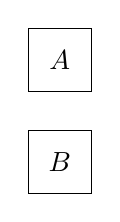
\begin{tikzpicture}
\draw (0,1.3)--(0.8,1.3)--(0.8,2.1)--(0,2.1)--cycle;
\node at (0.4,1.7) {$A$};
\draw (0,0)--(0.8,0)--(0.8,0.8)--(0,0.8)--cycle;
\node at (0.4,0.4) {$B$};
\end{tikzpicture}
\end{adjustbox}

Аксиома (1) не будет выполнена.

\underline{Другое опр.} (М. Концевич) (конкурирующее)

\begin{adjustbox}{max width=\linewidth}
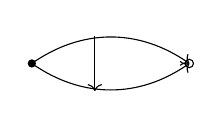
\begin{tikzpicture}[baseline=0cm]
\fill (0,0) circle (1.5pt);
\draw (2,0) circle (1.5pt);
\draw[->] (0,0) to[bend left=35] (2,0);
\draw[->] (0,0) to[bend right=35] (2,0);
\draw[->] (0.8,0.35)--(0.8,-0.35);
\end{tikzpicture}
\end{adjustbox}
морфизмы между морф. с одинаков. концами.

\underline{Пример:} $Cat$ (категория категорий; есть морфизм
функторов)

Это частный случай предыдущего (стягиваем верт. стрелки)

\underline{И.М.Г.}

\SourceFigure{GELFAND-P001406}{boundary-diagram}{В квадрате написано $\Delta u=0$. У верхней и нижней сторон горизонтальные стрелки направлены вправо; у левой стороны две внутренние вертикальные стрелки направлены вверх. Слева подписано $u$ и $\frac{\partial u}{\partial n}$; над этой подписью ещё одно неясное обозначение.}
гран. условия

Просьба к Келдышу — Ченцову — Гельфанду

\underline{К.} Высшие фунд. гр.
$X_0\subset X_1\subset X$ — топ. пр-во

объекты — точки $x\in X_0$

морф.
$\bigl(\underset{\text{отрезок}}{I},\partial I\bigr)\longrightarrow(X_1,X_0)$
\qquad гомотопные $(\mathrm{mod}\ \partial I)$ счит. эквив.

биморфизмы
$(I^2,\partial I^2)\longrightarrow(X,X_1)$
\qquad $(\mathrm{mod}\ \text{\underline{гомотопии}})$
% Review coordinates (original pixels): label [2220,20,2370,180];
% indices [390,950,1230,1160]; boundary diagram [245,2260,550,2455];
% cancelled groups [970,465,1050,530] and [1165,460,1300,565].

\SourcePage{GELFAND-P001407}{44}
\underline{\underline{23/XI-87 г.}} \qquad \underline{Сем. Гельфанда.}

\underline{Бейлинсон} (продолжение)

\underline{Производные категории.}

(1) \underline{Лемма:}
\begin{equation*}
\begin{adjustbox}{max width=\linewidth}
\begin{tikzcd}[column sep=small,row sep=small]
X^\bullet && Y^\bullet\\
& Z^\bullet \arrow[ul,"{\text{квази-изом.}}"] \arrow[ur] &
\end{tikzcd}
\end{adjustbox}
\quad\Rightarrow\quad\exists\quad
\begin{adjustbox}{max width=\linewidth}
\begin{tikzcd}[column sep=small,row sep=small]
& Z'^\bullet &\\
X^\bullet \arrow[ur,"{\text{квазиизом}}"] && Y^\bullet \arrow[ul]
\end{tikzcd}
\end{adjustbox}
\end{equation*}

Лемма док. с пом. конструкции конуса отображения.

\underline{Напоминание:}

$\mathcal{A}$ — аб. категория
\begin{equation*}
\begin{array}{ccccc}
C(\mathcal{A}) & \longrightarrow & K(\mathcal{A}) & \longrightarrow & D(\mathcal{A})\\
\text{комплексы} && \substack{\text{гомотоп.}\\\text{катег.}\\\text{комплексов}} &&
\substack{\text{производная}\\\text{категория}}
\end{array}
\end{equation*}
[Справа:] (объекты всюду суть комплексы)

$f:X^\bullet\to Y^\bullet$ гомотопно $0$, если
$\exists g^i:X^i\to Y^{i-1}$,
\begin{equation*}
f^i=dg^i+g^{i+1}d
\end{equation*}

$D(\mathcal{A})$ — это $K(\mathcal{A})$ с обращенными
\underline{квазиизоморфизмами}
(морф., индуц. изоморфизм когомологий)

Морфизм из $X^\bullet$ в $Y^\bullet$ — это диаграмма в $K(\mathcal{A})$
\begin{equation*}
\begin{adjustbox}{max width=\linewidth}
\begin{tikzcd}[column sep=small,row sep=small]
X^\bullet && Y^\bullet\\
& Z^\bullet \arrow[ul,"\sim"] \arrow[ur] &
\end{tikzcd}
\end{adjustbox}
\tag{2}
\end{equation*}
(левая стрелка — квазиизоморфизм)

точнее, класс эквивал. таких диаграмм: диагр. (2) эквивалентна
диаграмме, полученной с пом. любого квазиизоморфизма
$\chi:Z'^\bullet\to Z^\bullet$
\begin{equation*}
\begin{adjustbox}{max width=\linewidth}
\begin{tikzcd}[column sep=small,row sep=small]
X^\bullet && Y^\bullet\\
& Z^\bullet \arrow[ul,"\varphi"',"\sim"] \arrow[ur,"\psi"] &\\
& Z'^\bullet \arrow[u,"\chi"',"\sim"] &
\end{tikzcd}
\end{adjustbox}
\qquad
\begin{adjustbox}{max width=\linewidth}
\begin{tikzcd}[column sep=small,row sep=small]
X^\bullet && Y^\bullet\\
& Z' \arrow[ul,"{\varphi\circ\chi}"',"\sim"] \arrow[ur,"{\psi\circ\chi}"'] &
\end{tikzcd}
\end{adjustbox}
\tag{3}
\end{equation*}

(это отношение продолжается до наименьшего содержащего его
отношения эквивалентности)

Конус морфизма и точные треугольники были определены
[зачёркнуто: \Unclear{GELFAND-P001407}{last-line-cancellation}{неразборчиво}]
ещё.
% Review coordinates (original pixels): (1) [150,375,1370,735];
% (2) [290,1900,800,2200]; (3) [210,2320,1640,2760];
% final cancellation [1970,2925,2085,2990], inspected at 10x.
% Composition circles confirmed at 10x: [1195,2415,1335,2540] and
% [1450,2440,1610,2570].

\SourcePage{GELFAND-P001408}{unlabelled}
% Original image: 2408 x 3448 pixels. Coordinates below use the original pixel grid.
% Header and first example: (250,65)-(2150,745).
\underline{И. Захаревич}
[зачёркнуто: \Unclear{GELFAND-P001408}{cancelled-title}{неразборчиво}]
\underline{Импровизация \Unclear{GELFAND-P001408}{title-preposition}{о / с} хаосе.}

\underline{Примеры}

$1^{\circ}$. Видимо, есть морфизм из одного примера в другой.
\begin{equation*}
M=(\mathbb{Z}/2\mathbb{Z})^{\mathbb{Z}}
\qquad\text{(беск. в обе стороны послед.)}
\end{equation*}
$T\colon M\to M$. На $M$ станд. топология (кантор. мн-во).
\begin{equation*}
a_i\to a_{i-1}\qquad\text{(преобр. сдвига; преобр. Бернулли)}
\end{equation*}
Рассм. итерации: $T^N$.

% Baker transformation and cancellations: (300,725)-(2250,1590).
На $M$ есть мера. Преобр. пекаря совпадает с этим
[вставлено над строкой: (с точн. до меры $0$)]
[зачёркнуто после «этим» и строкой ниже:
\Unclear{GELFAND-P001408}{baker-cancellations}{неразборчиво}].

% Confidently visible labelled axes and folding arrow: (390,950)-(940,1285).
\begin{center}
\begin{adjustbox}{max width=\linewidth}
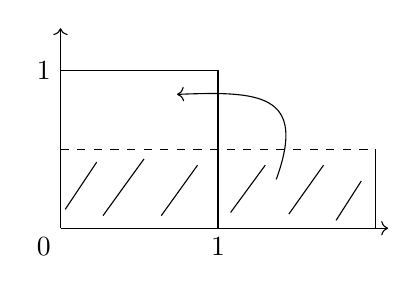
\begin{tikzpicture}[x=2cm,y=2cm]
\draw[->] (0,0) -- (2.08,0);
\draw[->] (0,0) -- (0,1.27);
\draw (0,1) -- (1,1) -- (1,0);
\draw (2,0) -- (2,0.5);
\draw[dashed] (0,0.5) -- (2,0.5);
\draw (0.03,0.12) -- (0.23,0.42);
\draw (0.27,0.08) -- (0.53,0.44);
\draw (0.64,0.08) -- (0.87,0.4);
\draw (1.08,0.1) -- (1.3,0.4);
\draw (1.45,0.09) -- (1.67,0.4);
\draw (1.75,0.05) -- (1.91,0.3);
\draw[->] (1.37,0.31) .. controls (1.57,0.86) and (1.26,0.87) .. (0.74,0.85);
\node[below left] at (0,0) {$0$};
\node[left] at (0,1) {$1$};
\node[below] at (1,0) {$1$};
\end{tikzpicture}
\end{adjustbox}
\end{center}

\SourceFigure{GELFAND-P001408}{baker-sequence}{Три рисунка слева направо: квадрат с замкнутой округлой кривой и горизонтальной пунктирной линией; квадрат с двумя вытянутыми изгибами, входящими с противоположных сторон; квадрат с несколькими почти горизонтальными полосами и короткими петлеобразными изгибами у краёв. В третьем рисунке различима стрелка влево на нижней длинной линии; направление мелких штрихов первого и третьего рисунков не вполне ясно.}
и т. д.

% Binary correspondence and forward/backward iterates: (295,1590)-(2230,2260).
\underline{Соответствие}: записать коорд. точки квадрата в двоичной системе
и взять $1$ цифру — налево, другую — направо.

В каком смысле это хаос

Рассм. $T^k x$, $k\leq 0$ — пусть это известно (с точн. до $1$ мм).
\begin{equation*}
T^k x,\qquad k>0
\end{equation*}
за конечное время вся эта информ. потеряется.

% Second example: (305,2290)-(2400,2700).
$2^{\circ}$. \underline{Гиперболич. преобразование}:
геодезич. потоки на \Unclear{GELFAND-P001408}{manifold-abbreviation}{мн-зиях / мн-иях} отриц. кривизны.

\SourceFigure{GELFAND-P001408}{hyperbolic-surface}{Замкнутый контур с двумя расширениями и перетяжкой между ними. Внутри слева и справа нарисованы дуги, похожие на обозначения двух ручек поверхности; в средней части короткий наклонный отрезок с выделенными концами и ответвляющейся стрелкой вправо-вверх. Мелкие направления и точное соединение внутренних дуг требуют проверки оригинала.}

\SourcePage{GELFAND-P001409}{45}
% Original image: 2408 x 3448 pixels. All coordinates refer to original pixels.
% Header: (205,35)-(2280,200).
\underline{Г. Маргулис.}
\underline{Итерации отображений компл. плоскости.}

Рассм. преобр. $z\to P(z)$, $P$ — многочлен

(более общо — рац. ф-я)

$\operatorname{deg}P=1$
[зачёркнуто: \Unclear{GELFAND-P001409}{degree-one-cancellation}{неразборчиво}]
неинтересный случай

$(1)\quad z\mapsto az+b$

\underline{Итерации}:
\begin{equation*}
z_{i+1}=P(z_i)
\end{equation*}
$|a|>1\Rightarrow$ одна неподв. точка;

\Unclear{GELFAND-P001409}{unit-modulus-claim}{$|a|=1\Rightarrow$ всё разбив. на инвар. окружности, на к-рых поворот.}

% Three nested circular contours with a central point: (265,985)-(580,1235).
\begin{center}
\begin{adjustbox}{max width=\linewidth}
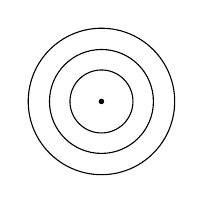
\begin{tikzpicture}
\draw (0,0) circle (0.4);
\draw (0,0) circle (0.66);
\draw (0,0) circle (0.93);
\fill (0,0) circle (0.035);
\end{tikzpicture}
\end{adjustbox}
\end{center}

% Gelfand interjection: (135,1240)-(2340,1745).
\underline{И. М. Г.}: 1) вопрос о том, когда преобраз. окружности диффеоморфно повороту,
нетривиален: Данжуа, Арнольд, Herman

2) Что такое представление дискретной бескон. группы?

Нет удовлетв. ответа.

Фон Неймановская теор. не эстетична.

На окружности возникает хаос.

\underline{Гипотеза}: если работать с мн-вами промежуточной хаусдорфовой
размерности, то нек-рая классика восстановится!!

% Covering question and tasks: (100,2070)-(2340,2820).
\underline{Вопрос для школьников}: покрываем $n$-е рац. число интервалом
длины $\varepsilon/2^n$. Привести пример числа, к-рое не будет покрыто.

\underline{Задача}: найти хаусд. размерность канторовского соверш. мн-ва.

\tikz\node[draw,circle,inner sep=2pt] {!};
\underline{Задача}. \underline{Построить теорию предст. дискр. групп на ф-ях на}
\underline{мн-вах промежут. хаусд. размерности.}

Для начала посмотреть физику — теор. струн и т. д.

% Margulis resumes: (170,2800)-(2180,3230).
\underline{Г. М.}:
$z\to z^2$
\qquad $|z|=1$ перех. в себя

\begin{center}
\begin{adjustbox}{max width=\linewidth}
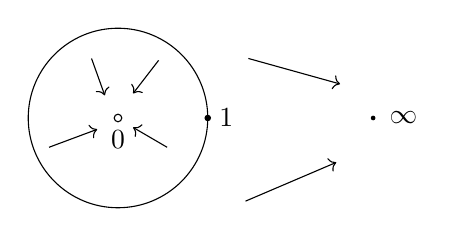
\begin{tikzpicture}[x=1.2cm,y=1.2cm]
\draw (0,0) circle (0.95);
\draw (0,0) circle (0.04);
\node[below] at (0,-0.03) {$0$};
\fill (0.95,0) circle (0.035);
\node[right] at (0.97,0) {$1$};
\draw[->] (-0.28,0.63) -- (-0.14,0.24);
\draw[->] (0.43,0.61) -- (0.16,0.26);
\draw[->] (0.52,-0.31) -- (0.16,-0.1);
\draw[->] (-0.73,-0.31) -- (-0.22,-0.12);
\draw[->] (1.38,0.63) -- (2.35,0.36);
\draw[->] (1.35,-0.88) -- (2.31,-0.47);
\fill (2.7,0) circle (0.025);
\node[right] at (2.77,0) {$\infty$};
\end{tikzpicture}
\end{adjustbox}
\end{center}
на окр. — аналог преобр. пекаря
(одностороннего)

\SourcePage{GELFAND-P001410}{unlabelled}
% Original image: 2408 x 3448 pixels. Coordinates use the original pixel grid.
% Iteration and normality definition: (140,40)-(2360,900).
\begin{equation*}
f_n=\underbrace{f\circ f\circ\cdots\circ f}_{n\ \text{раз}}
\end{equation*}
\underline{Опр.}

$U$ — [зачёркнуто: мн-во; над строкой вставлено: окр.]
нормальности; если $\left.f_n\right|_U$ — компактное мн-во

(норм. сем-во анал. ф-й)

[На отдельной короткой строке зачёркнуто:
\Unclear{GELFAND-P001410}{isolated-cancellation}{неразборчиво}.]

Мн-во норм. [вставлено над строкой: $X$] сост. из точек $x$, для к-рых
$\exists$ окр. $U$ — [зачёркнуто:
\Unclear{GELFAND-P001410}{normality-cancellation}{неразборчиво}]
окр. нормальности

[Под «Мн-во норм.»: (оно открыто)]

Дополнение к мн-ву нормальности — \underline{мн-во Жюлиа}.

(оно замкнуто)

Мн-во норм. может быть пусто

% Components and Sullivan's assertion: (160,900)-(2130,1790).
\begin{equation*}
X=X_1\cup\cdots\cup X_n\cup\cdots
\end{equation*}
(связные компоненты)

мн-ва нормальности

[зачёркнуто под этой подписью:
\Unclear{GELFAND-P001410}{components-cancellation}{неразборчиво}]

\begin{equation*}
\begin{aligned}
f\colon (\text{св. компон.})&\to(\text{св. компоненты})\\
X_i&\mapsto X_{j(i)}
\end{aligned}
\end{equation*}
\underline{Sullivan} доказал, что в возникающем

[зачёркнуто: \Unclear{GELFAND-P001410}{sullivan-cancellation}{неразборчиво}]
преобр. дискр. мн-ва (счётн. или конечного)

а) каждая орбита стабилизируется,

б) мн-во неподв. точек конечно.

\underline{Идея док-ва}. Пусть есть беск. орбита

% Five ovals with interior small circles; lower labels only 1,2,3,4: (335,1925)-(1195,2105).
\begin{center}
\begin{adjustbox}{max width=\linewidth}
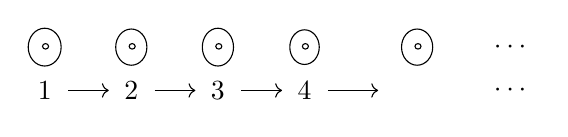
\begin{tikzpicture}[x=1.1cm,y=1cm]
\draw (0,0) ellipse (0.19 and 0.24);
\draw (0.01,0.01) circle (0.035);
\draw (1,0) ellipse (0.18 and 0.23);
\draw (1.01,0.01) circle (0.035);
\draw (2,0) ellipse (0.18 and 0.24);
\draw (2.01,0.01) circle (0.035);
\draw (3,0) ellipse (0.17 and 0.22);
\draw (3.01,0.01) circle (0.035);
\draw (4.3,0) ellipse (0.18 and 0.23);
\draw (4.31,0.01) circle (0.035);
\node at (5.4,0) {$\cdots$};
\node at (0,-0.55) {$1$};
\node at (1,-0.55) {$2$};
\node at (2,-0.55) {$3$};
\node at (3,-0.55) {$4$};
\draw[->] (0.27,-0.55) -- (0.74,-0.55);
\draw[->] (1.27,-0.55) -- (1.74,-0.55);
\draw[->] (2.27,-0.55) -- (2.74,-0.55);
\draw[->] (3.27,-0.55) -- (3.85,-0.55);
\node at (5.4,-0.55) {$\cdots$};
\end{tikzpicture}
\end{adjustbox}
\end{center}

Сделаем замену конф.
[зачёркнуто: \Unclear{GELFAND-P001410}{structure-cancellation}{преобр. / неразборчиво}]
структуру, чтобы преобр. осталось
конформным.

% Packing problem and its two requests: (245,2330)-(1880,2950).
\underline{Задача}:

\SourceFigure{GELFAND-P001410}{circle-packing}{В квадрате нарисованы четыре больших округлых контура, по два в верхнем и нижнем рядах; в промежутках и у границы имеются меньшие замкнутые кривые. Справа в сторону квадрата направлена горизонтальная стрелка с подписью «вписываем». Точные касания и принадлежность мелких пограничных дуг отдельным контурам не вполне различимы.}

1) Док., что остаток имеет меру $0$

2) Док., что остаток имеет хаусд. размерность $<2$.

\SourcePage{GELFAND-P001411}{46}
% Original frame: 2408 x 3448. Heading bbox (190,40,1500,195); label (2160,35,2340,140).
\underline{\underline{И.М. Гельфанд}}. \underline{Матроиды.}

% Original text bbox (205,190,2290,630); inspected in 3x crops.
В $K$-мерном пр-ве рассм. $n$ векторов;
занумеруем их и составим список: какие лин. завис., а какие — нет.
Задание этого списка — \underline{матроид}.

Какие условия на этот список?

\underline{Пример}:
[Зачёркнуто: \Unclear{GELFAND-P001411}{example-cancelled}{неразборчиво}.]

% Figure bbox (305,678,590,882), enlarged 6x. Seven marked points; two solid and five outlined.
\begin{center}
\begin{adjustbox}{max width=\linewidth}
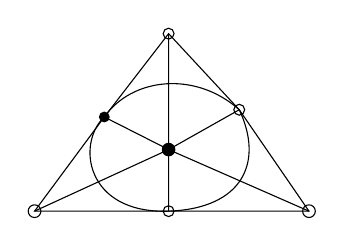
\begin{tikzpicture}[scale=1.15]
\coordinate (a) at (0,1.96);
\coordinate (b) at (-1.48,0);
\coordinate (c) at (1.55,0);
\coordinate (d) at (-0.71,1.04);
\coordinate (e) at (0.78,1.12);
\coordinate (f) at (0,0);
\coordinate (g) at (0,0.68);
\draw (a)--(d)--(b)--(f)--(c)--(e)--cycle;
\draw (a)--(g)--(f) (b)--(g)--(e) (d)--(g)--(c);
\draw (d) .. controls (-0.40,1.48) and (0.30,1.55) .. (e)
 .. controls (1.05,0.55) and (0.83,0.03) .. (f)
 .. controls (-0.92,-0.03) and (-1.02,0.75) .. (d);
\draw (a) circle (0.06) (b) circle (0.07) (c) circle (0.07)
 (e) circle (0.06) (f) circle (0.06);
\fill (d) circle (0.06) (g) circle (0.075);
\end{tikzpicture}
\end{adjustbox}
\end{center}

если 3 точки лежат на одной линии, то векторы
линейно зависимы.

Всё пр-во 3-мерно (нет 4-х лин. независимых)

% Original bbox (90,985,2270,1640), inspected at 3x.
(1) \underline{Задача}: 1) док., что над $\mathbb{R}$ и $\mathbb{C}$ таких векторов нет!

2) над $\mathbb{Z}/2\mathbb{Z}$ такие векторы есть.

(все ненулевые векторы у $(\mathbb{Z}/2\mathbb{Z})^3$!)

\underline{Общая} (\underline{нереш. задача}): какие матроиды реализуются
а) над $\mathbb{R}$
б) над $\mathbb{C}$.?

\underline{Решена задача}: какие матроиды реализ. над $\forall$ полем?

% Book reference bbox (190,1810,1750,2025), word enlarged 5x; glyph after Рота enlarged 7x.
\underline{В книжке Рота} \Unclear{GELFAND-P001411}{book-after-rota}{э..}
[Справа: см. \Unclear{GELFAND-P001411}{book-overwritten-noun}{книге?} \underline{Айгнера} (?)]
имеется 15 различных эквив. опр. матроида.

% Original bbox (75,2020,2280,2550); cancellation (1470,2315,1650,2450), enlarged 8x.
(2) \underline{Аксиоматика}.

Выделены подмн-ва, \underline{называемые базисами}

$B_1,B_2$ — 2 базиса

$y\in B_2,\ y\notin B_1\ \Rightarrow\ \exists x\in B_1;$
$(B_1\setminus x)\cup y$
[Зачёркнуто: \Unclear{GELFAND-P001411}{basis-exchange-cancelled}{неразборчиво}],
$(B_2\setminus y)\cup x$ —
\newline
— базисы

\underline{Упр. из лин. алгебры}: проверить для мн-ва векторов в лин. пр-ве.

% Original bbox (50,2670,2370,3425); definition enlarged 4x and 6x.
(3) \underline{Биматроид}: рассм. матрицу; из неё опр. 2 матроида — по столбцам
и строкам

$S$ и $T$

Другое понятие: выписать все миноры $\ne0$

Биматроид: набор подмн-в с одинак. числом элементов.

(4) [Зачёркнуто: \Unclear{GELFAND-P001411}{problem-four-cancelled}{неразборчиво}.]
\underline{Задача}: указать аксиомы для биматроида.

\SourcePage{GELFAND-P001412}{unlabelled}
% Original frame: 2408 x 3448; no confidently visible page label.
% Top bbox (115,55,2370,315), enlarged 3x; name (550,160,875,285), enlarged 8x.
(5) \underline{Задача}: как понятие биматроида из
[Зачёркнуто: \Unclear{GELFAND-P001412}{top-cancelled}{неразборчиво}]
Гельфанда — Сергановой (УМН)
связано с \Unclear{GELFAND-P001412}{knuth-name}{Кунтом}

\underline{Задача}: доказать, что

% Formula bbox (275,270,2320,425), inspected at 3x, 6x and 8x. Keep anomalous indices/sign as seen.
\begin{equation*}
\text{(6)}\quad
[x_1,\ldots,x_d][y_1,\ldots,y_d]
=\sum(-1)^{d-i}[y_1,x_2,\ldots,x_d]
[y_1,\ldots,y_{i-1},x_i,y_{i+1},\ldots,y_d]
\end{equation*}
\Unclear{GELFAND-P001412}{determinant-formula-source}{индексы $y_1$, $x_i$ и знак $(-1)^{d-i}$ — по рукописи}

$[x_1,\ldots,x_d]$ — детерминант, постр. по вект.

% Original bbox (105,580,2270,810), inspected 3x.
(7) \underline{Замеч.}: если $[x_1,\ldots,x_d]$, $[y_1,\ldots,y_d]$ — базисы, то справа есть
ненулевое слагаемое — это и даёт аксиому замены
\Unclear{GELFAND-P001412}{basis-axiom-reference}{(3)}

% Chain bbox (125,880,2245,1220), inspected 3x; overwritten numeral 8x.
(\Unclear{GELFAND-P001412}{overwritten-eight}{8})
\underline{Задача} (нудная). Цепь сизигий по Гильберту:
\begin{equation*}
(\text{кольцо})\longmapsto
\underset{\text{— детерминанты}}{(\text{образующие})}
\longmapsto (\text{соотн. между образующими})
\end{equation*}

% Original bbox (90,1195,2210,1525), inspected 3x.
(9) (\underline{Утв.}: (6) — все соотн. между образующими)

(10) а) Написать всю цепочку!

б) Дискретизовать (комбинат. соотн. написать) всей цепочки.

% Original bbox (120,1570,2370,2150), inspected 3x; cancellation enlarged 8x.
(11) \underline{Задача}. Биматроид — список миноров $\longrightarrow$
[Зачёркнуто: \Unclear{GELFAND-P001412}{problem-eleven-cancelled}{неразборчиво}]
2 матроида
(стр. и столбцы)

По 2-м матроидам строится биматроид

\SourceFigure{GELFAND-P001412}{basis-grid}{Решётка из четырёх вертикальных и четырёх горизонтальных линий; слева и снизу фигурные скобки с подписями «баз…»; справа стрелка направлена влево, к решётке.}

по опр. \Unclear{GELFAND-P001412}{basis-construction-word}{база?}.

% Lower prose bbox (275,2130,2220,2810), inspected 3x; last adjective enlarged 6x.
Но это не обязательно.

В биматроиде больше информации.

Какова доп. информация в биматроиде?

Это важное когомологич. понятие.

\underline{Замеч.} Алгебр. топология — маленький остров в привычной
комбинат. технике.

\SourcePage{GELFAND-P001413}{unlabelled}
% Оригинал: 2408 x 3448. Координаты обзора (x0,y0,x1,y1), начало слева сверху:
% заголовок 150,65,2160,375; Керов и образующие 165,365,2230,605;
% (1) 280,600,1700,1010; (2)--(4) 80,1010,2300,1670;
% библиография 135,1700,2335,2470; конструкция и (5) 200,2530,2050,3280.
% Текстовые сомнения проверены увеличениями 3--5x, малые знаки 4--5x.
\underline{\underline{30/XI-87г.}}\qquad \underline{Сем. Гельфанда.}

\underline{И.М. Гельфанд.} Задача: найти характеры симметрической группы.

(по следам Фробениуса).

\underline{О раб.} \underline{Керова}: «\underline{Реализация предст. алгебры Геке} и т.д.»

Подсказка: это характеры симм. группы.

Алгебра Геке --- алгебра с образующими $\{e_k\}$
[над строкой: $k=1,\ldots,N-1$] и соотношениями
\begin{equation*}
\text{(1)}\quad
\left\{\begin{aligned}
e_k e_{k+1}e_k-\tau e_k&=e_{k+1}e_k e_{k+1}-\tau e_{k+1}\\
e_{k+j}e_k&=e_k e_{k+j},\quad j\geq 2;\\
e_k^2&=e_k
\end{aligned}\right.
\end{equation*}
Другие образующие
\begin{equation*}
\text{(2)}\quad \sigma_k=(q+1)e_k-1,\qquad \tau=\frac{q}{(q+1)^2}
\end{equation*}
Эта алг. обозначена $H_N(q)$.

\underline{Упражнение}: записать соотношения на $\sigma_k$.

(3) При $q=1$ (или $\tau=\frac14$) получается групповая алгебра симм. группы.

(4) \underline{Задача}: $\dim H_N(q)=N!$

[На левом поле: обведённый в круг «!».]
В работе \Unclear{GELFAND-P001413}{citation-name}{Типпера / Диппера} и Джеймса

Proc. London Math. Soc.\qquad 1986, v. 52, p. 20--52

рекомендуется!!

док., что теория предст. $H_N(q)$ аналогична теории модулярных
предст. симметрической группы.

Это работает даже в комплексном случае (см. раб. Бернш.--Гельф.--Гельф.
о модулях Верма).

При этом предполагается, что $q\ne\sqrt[m]{1}$

\underline{Конструкция представлений.}

Диаграмма Юнга\quad $\lambda=(\lambda_1,\lambda_2,\ldots,\lambda_k)$

\begin{center}
(5)\qquad
\begin{adjustbox}{max width=\linewidth}
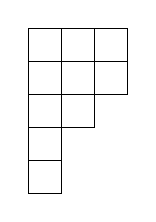
\begin{tikzpicture}[x=0.42cm,y=0.42cm]
\draw (0,0)--(3,0)--(3,-2)--(2,-2)--(2,-3)--(1,-3)--(1,-5)--(0,-5)--cycle;
\draw (1,0)--(1,-5);
\draw (2,0)--(2,-3);
\draw (0,-1)--(3,-1);
\draw (0,-2)--(3,-2);
\draw (0,-3)--(2,-3);
\draw (0,-4)--(1,-4);
\end{tikzpicture}
\end{adjustbox}
\qquad
$\begin{gathered}\sum\lambda_j=|\lambda|\\[8pt]\lambda_{i+1}\leq\lambda_i\end{gathered}$
\end{center}

($\lambda_i$ --- число клеток в $i$-м столбце)

Это соотв. классу сопряж. элементов.

\SourcePage{GELFAND-P001414}{52}
% Оригинал: 2408 x 3448. Координаты обзора (x0,y0,x1,y1), начало слева сверху:
% (6) 110,30,2200,410; определение и большая таблица 80,410,2250,890;
% три малые таблицы 130,940,1090,1290; (7)--(9) 100,1290,2220,2295;
% (10)--(12) 110,2330,1910,2940; (13)--(14) 65,2930,2030,3448.
% Неясные слова/штрихи просмотрены при 3--10x; новых исходных пикселей нет.
Таблица Юнга:
\begin{equation*}
\text{(6)}\quad t=\{\lambda^{(k)}\}_{k=1}^{N}
\quad\text{--- набор диаграмм, в котором}
\end{equation*}
\begin{equation*}
|\lambda^{(k)}|=k.
\end{equation*}

Обычное опред. (другое): табл. заполн. числами $1,2,\ldots,|\lambda|$, причём
\begin{equation*}
\begin{matrix}\rightarrow\\\downarrow\end{matrix}
\quad\text{по этим напр. возрастание}
\end{equation*}

% Контур большой таблицы воспроизведён без добавления внутренних линий:
% в источнике подписаны 1,2,4,7 / 3,5,8 / 6, нижняя часть длинной ножки пустая.
\begin{center}
\begin{adjustbox}{max width=\linewidth}
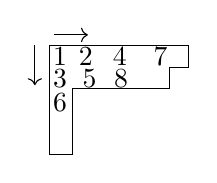
\begin{tikzpicture}[x=0.44cm,y=0.44cm]
\draw (0,0)--(4,0)--(4,-0.65)--(3.45,-0.65)--(3.45,-1.25)--(0.65,-1.25)--(0.65,-3.15)--(0,-3.15)--cycle;
\node at (0.30,-0.33) {$1$};
\node at (1.04,-0.33) {$2$};
\node at (2.02,-0.33) {$4$};
\node at (3.20,-0.33) {$7$};
\node at (0.30,-0.97) {$3$};
\node at (1.15,-0.97) {$5$};
\node at (2.06,-0.97) {$8$};
\node at (0.30,-1.66) {$6$};
\draw[->] (0.12,0.30)--(1.10,0.30);
\draw[->] (-0.43,0.0)--(-0.43,-1.15);
\end{tikzpicture}
\end{adjustbox}
\end{center}

В (6) они должны возрастать

\begin{center}
\begin{adjustbox}{max width=\linewidth}
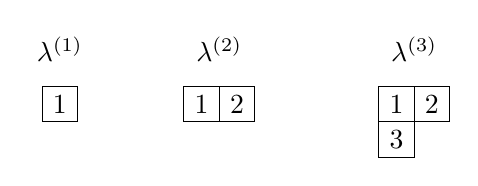
\begin{tikzpicture}[x=0.45cm,y=0.45cm]
\node at (0.5,1.05) {$\lambda^{(1)}$};
\draw (0,0) rectangle (1,-1);
\node at (0.5,-0.5) {$1$};
\node at (5,1.05) {$\lambda^{(2)}$};
\draw (4,0) rectangle (6,-1);
\draw (5,0)--(5,-1);
\node at (4.5,-0.5) {$1$};
\node at (5.5,-0.5) {$2$};
\node at (10.5,1.05) {$\lambda^{(3)}$};
\draw (9.5,0)--(11.5,0)--(11.5,-1)--(10.5,-1)--(10.5,-2)--(9.5,-2)--cycle;
\draw (10.5,0)--(10.5,-1);
\draw (9.5,-1)--(10.5,-1);
\node at (10,-0.5) {$1$};
\node at (11,-0.5) {$2$};
\node at (10,-1.5) {$3$};
\end{tikzpicture}
\end{adjustbox}
\end{center}

\begin{equation*}
\text{(7)}\quad r_k(t)=(i_{k+1}-j_{k+1})-(i_k-j_k)
\end{equation*}
точка $k$ имеет координаты $(i_k,j_k)$

Для диаграммы:
\begin{equation*}
\text{(8)}\quad h(\lambda)=r_\lambda+1
\end{equation*}
\begin{equation*}
\text{(9)}\quad r_\lambda=\max_{t\in T(\lambda)}\max_{1\leq k<N}|r_k(t)|,
\end{equation*}
где $T(\lambda)$ --- мн-во таблиц, построенных по диаграмме $\lambda$, т.е.
имеющих форму $\lambda$.

Пусть $s=(\mu^{(k)})_{k=1}^{N}$,\quad $t=(\lambda^{(k)})_{k=1}^{N}$.

(10) \underline{Опр.}\quad $s\underset{n}{\approx}t$, если $\lambda^{(k)}=\mu^{(k)}$, $k\ne n$

\underline{Утверждение.}

(11) [Зачёркнуто: \Unclear{GELFAND-P001414}{eq11-cancelled-word}{если?};
над строкой вставлено: Пусть]
$r_n(t)=\pm1$; тогда $s\underset{n}{\approx}t\Rightarrow s=t$;

(12) Пусть $|r_n(t)|>1$; тогда $\exists!\ s:\quad s\underset{n}{\approx}t$, $s\ne t$.

\begin{equation*}
\text{(13)}\quad S_\lambda^{(k)}=\Vert S_{s,t}^{(k)}(\tau)\Vert_{s,t\in T(\lambda)}
\quad\text{--- матрица};
\end{equation*}
[После индекса у матрицы, ниже строки:
\Unclear{GELFAND-P001414}{eq13-terminal-mark}{неразборчивый знак; $q$ / исправленная запятая}.]

\begin{equation*}
\text{(14)}\quad
S_{s,t}^{(k)}(\tau)=\bigl(W_{r_k(s)}(\tau)\ W_{r_k(t)}(\tau)\bigr)^{1/2}
\quad\text{при }s\underset{k}{\approx}t
\end{equation*}
[После первого множителя, ниже строки:
\Unclear{GELFAND-P001414}{eq14-blotted-mark}{замазанный или зачёркнутый знак}.]

[Зачёркнуто: \Unclear{GELFAND-P001414}{eq14-cancelled-condition}{при $s\underset{k}{\approx}t$?}]
и $S_{s,t}^{(k)}(\tau)=0$ в противном случае.


\SourcePage{GELFAND-P001415}{unlabelled}
(15) \underline{Теорема}. Пусть $\lambda$ — диаг. из $N$ элементов и
$q\ne\sqrt[m]{1}$. Тогда $S_{\lambda}^{(k)}$ задают представление алгебры Гекке
(в образующих $e_k$).

Построим ф-и $W$.
$W_{-r}(\tau)$ при $r=1,2,\ldots$ опред. из соотношений
\begin{equation}
 W_{-(r+1)}(\tau)=1-\frac{\tau}{W_{-r}(\tau)},\qquad r\geq0,
 \tag{16}
\end{equation}
[Зачёркнуто: \Unclear{GELFAND-P001415}{eq16-cancelled}{а при $r\ne0$; возможно, $r\geq0$.}]
\begin{equation}
 W_r(\tau)=1-W_{-r}(\tau),\qquad r\geq0;
 \tag{17}
\end{equation}

Или:

$W_{-r}(\tau)$ опр.
[Зачёркнуто: \Unclear{GELFAND-P001415}{continued-fraction-cancelled-word}{неразборчиво}]
из разл. в цепную дробь:
\begin{equation}
 \text{[Зачёркнуто: }W_{-r}(\tau)=\text{]}\quad
 1-\frac{\tau}{1-\dfrac{\tau}{1-\ldots}}
 \tag{18}
\end{equation}
Имеется ур-е:
\begin{equation}
 W_r(\tau)W_{1-r}(\tau)=1.
 \tag{19}
\end{equation}
\Unclear{GELFAND-P001415}{eq19-right-hand-side}{В правой части написано $1$.}

Общая ф-ла:
\begin{equation}
 W_r(\tau)=\frac{q(q^{r-1}-1)}{(q+1)(q^r-1)},\qquad r=1,2,\ldots
 \tag{20}
\end{equation}
\begin{equation}
 W_{-r}(\tau)=\frac{q^{r+1}-1}{(q+1)(q^r-1)}.
 \tag{21}
\end{equation}
\Unclear{GELFAND-P001415}{w-index}{Индекс функций $W$: $r$; возможно, $i$.}

(22) \underline{Задача}: найти характеры алгебры Гекке.

Рассмотрим
\begin{equation}
 \frac{
 \begin{vmatrix}
 x_1^{i_1}&x_1^{i_2+1}&\ldots&x_1^{i_n+n-1}\\
 x_2^{i_1}&x_2^{i_2+1}&\ldots&x_2^{i_n+n-1}\\
 \ldots&\ldots&\ldots&\ldots\\
 x_n^{i_1}&\ldots&\ldots&x_n^{i_n+n-1}
 \end{vmatrix}
 }{
 \begin{vmatrix}
 1&x_1&x_1^2&\ldots&x_1^{n-1}\\
 1&x_2&x_2^2&\ldots&\\
 \ldots&\ldots&\ldots&\ldots&\\
 1&x_n&x_n^2&\ldots&x_n^{n-1}
 \end{vmatrix}
 }
 =\sum a(i,j)P_{j_1}P_{j_2}\ldots P_{j_n}
 \tag{23}
\end{equation}
\Unclear{GELFAND-P001415}{eq23-overwritten-exponents}{В первых двух строках последнего столбца числителя: $i_n+n-1$; нижний индекс у $i$ исправлен поверх прежних штрихов.}

\SourcePage{GELFAND-P001416}{53}
$j=(j_1,\ldots,j_n)$, $P_j$ — сумма степеней.

Тогда

(24) $a(i,j)$ — знач. характера [вставлено над строкой: симм. группы]
на элем. с длинами циклов $j_1,\ldots,j_n$

(с точн. до простой константы)

По поводу симм. группы см. книгу Макдональда «Симм. ф-и
и многочлены Холла».

\medskip
\underline{Локализация полюсов у дзета-функции Рюэлля.}

(\Unclear{GELFAND-P001416}{mayer-name}{Линдон Майер (?)})

Letters in Math. Physics, $14:2$, 1987 г.

$I$ — интервал, $T:I\to I$ — кусочно линейное
\begin{equation*}
 I=\bigcup_j I_j,\qquad T(I_j)=I.
\end{equation*}
\SourceFigure{GELFAND-P001416}{interval-graph}{Прямоугольная рамка без подписей; внутри несколько восходящих наклонных ветвей и почти вертикальных штрихов. Принадлежность коротких штрихов ветвям и точное число разрывов требуют сверки с оригиналом.}

\begin{equation}
 \zeta_T(z,\varphi)=\frac{\det(1-zL_1)}{\det(1-zL_2)},
 \tag{1}
\end{equation}
где
\begin{equation*}
 L_1f(z)=\varphi(z)\sum\frac{1}{\rho_j}f(\psi_j(z)),
\end{equation*}
\begin{equation*}
 L_2f(z)=\varphi(z)\sum f(\psi_j(z)),
\end{equation*}
$\psi_j$ — локальные обратные $T$ на интервале $I_j$, а $\rho_j^{-1}$ — наклон.
\Unclear{GELFAND-P001416}{slope-letter}{Буква в $\rho_j$ допускает также чтение $p_j$.}

В общем случае:
\begin{equation}
 \zeta_T(z,\varphi)=
 \exp\left(
 \sum_{n=1}^{\infty}\frac{z^n}{n}
 \sum_{\xi\in\mathrm{Fix}\,T^n}
 \prod_{k=0}^{n-1}\varphi(T^k x)
 \right)
 \tag{2}
\end{equation}
\Unclear{GELFAND-P001416}{eq2-variable}{Под второй суммой написано $\xi\in\mathrm{Fix}\,T^n$, в произведении — $x$.}

\SourcePage{GELFAND-P001417}{unlabelled}
\underline{7/XII-87.}\qquad \underline{Сем. Гельфанда!}\qquad Нечто о работе

\underline{D. Mayer}\qquad \underline{Lett. in Math. Phys. 1987, $14:2$}

\underline{О $\zeta$-функции Рюэлля}

$F$ — мн-во значений спина (конечное).

Изучаем конфигурации спина на решётке
\begin{equation*}
 (\xi_i),\qquad -\infty<i<\infty,\qquad \xi_i\in F.
\end{equation*}
$M\subseteq F\times F$ — допустимое мн-во; требуется, чтобы было
\begin{equation}
 (\xi_i,\xi_{i+1})\in M.
 \tag{1}
\end{equation}

Простейший пример рюэллевской $\zeta$-ф-и — $\zeta$-ф-я Артина и Мазура.

Рассм. мн-во периодических конфигураций и их количество:
\begin{equation}
 N_n=\#\{(\xi_i)\mid\mathcal T^n(\xi_i)=(\xi_i)\}
 =\mathrm{Fix}\,\mathcal T^n,
 \tag{2}
\end{equation}
где $\mathcal T$ — преобр. в пр-ве послед.
\begin{equation*}
 \mathcal T(\xi_i)=\xi_{i+1}
\end{equation*}
(сдвиг)

$\zeta$-ф-я Рюэлля:
\begin{equation}
 \zeta_{\mathcal T}(s)=\exp\left(\sum_{n=1}^{\infty}\frac{N_n}{n}s^n\right)
 \tag{3}
\end{equation}
ряд сходится при $|s|<\dfrac{1}{|F|}$.

\Unclear{GELFAND-P001417}{continuation-question-overwriting}{Сущ. ли аналитическое продолжение? [Конец «Сущ.» и начальная «а» обведены поверх прежних штрихов.]}
Рассм. матрицу
\begin{equation}
 T=(T_{\alpha\beta})=
 \begin{cases}
 1,&(\alpha,\beta)\in M,\\
 0,&(\alpha,\beta)\notin M.
 \end{cases}
 \tag{4}
\end{equation}

Тогда
\begin{equation}
 \zeta_{\mathcal T}(s)=\frac{1}{\det(1-sT)}
 \tag{5}
\end{equation}

Отсюда видно, что $\zeta_{\mathcal T}(s)$ мероморфна.

Радиус сход. может быть больше, чем $1/|F|$.

Для док-ва нужно заметить, что
\begin{equation}
 N_n=\mathrm{Tr}\,T^n.
 \tag{6}
\end{equation}

\SourcePage{GELFAND-P001418}{62}
\underline{Замеч. И.М.Г.}: это похоже на раб. Дынкина и Дмитриева:
рассм. стох. матрицу $(p_{ik})$ [вставлено сверху: (стохастическую)]
(в задаче о бассейнах это
[зачёркнутый знак: \Unclear{GELFAND-P001418}{basin-cancelled-sign}{неразборчиво}]
доля воды, перелив. из $i$-го басс. в $k$-й).
\begin{equation*}
 \underline{P}=(p_{ik}),\qquad \sum_k p_{ik}=1.
\end{equation*}
Это зависит от соб. значений $P$.

а) Соб. значения лежат в круге $|\lambda|\leq1$,

б) $1$ — соб. значение.

Какую обл. заполняют соб. значения?

Это внутр. нек-рой алг. кривой.

Они делали неправильно.

Есть набор соб. значений!!

и надо рисовать набор соб. значений в $\mathbb C^n$ — это должна
быть красивая область (\underline{Задача!!})

Проекция на одну ось может быть сложной!

[Слева двойная черта; следующие две строки подчёркнуты:]
\underline{В задаче Рюэлля интересно посмотреть все соб. значения}

\underline{матрицы $T$.}

\medskip
\underline{Докладчик}. Обобщение примера (3)
\begin{equation}
 \zeta_{\mathcal T}(s;\varphi)=
 \exp\left(
 \sum_{n=1}^{\infty}\frac{s^n}{n}
 \sum_{\xi\in\mathrm{Fix}(\mathcal T^n)}
 \prod_{\ell=0}^{n}\varphi(\mathcal T^\ell\xi)
 \right)
 \tag{7}
\end{equation}
\Unclear{GELFAND-P001418}{eq7-upper-product-bound}{Верхний предел произведения написан как $n$.}

Здесь
\begin{equation*}
 \varphi=\varphi(\xi_1,\ldots,\xi_k),\qquad \xi_j\in F
\end{equation*}
[Под $\varphi$ черта к подписи: функция.]

($\varphi$ берётся только от первых $k$ значений).

((3) получается при $\varphi=1$)

(8) \underline{Утв.} $\exists$ [зачёркнуто: оператор; над строкой вставлено: матрица]
$L$ (конечномерная), такая что:
\begin{equation}
 \zeta_{\mathcal T}(s,\varphi)=\frac{1}{\det(1-sL)}
 \tag{9}
\end{equation}

А именно, рассм.
\begin{equation*}
 F'=F^k;
\end{equation*}
[Зачёркнуто: \Unclear{GELFAND-P001418}{before-m-prime-cancelled}{неразборчивая запись перед $M'$}.]
\begin{equation*}
 M'\subset F'\times F'
\end{equation*}
\begin{equation}
 M'=\{(\xi_1,\ldots,\xi_k);(\xi_2,\ldots,\xi_{k+1})
 \mid(\xi_i,\xi_{i+1})\in M\}
 \tag{10}
\end{equation}
\Unclear{GELFAND-P001418}{eq10-overwritten-indices}{Во втором кортеже индексы $2$ и $k+1$ исправлены; в условии $i+1$ также обведён.}

Тогда надо взять
\begin{equation*}
 \ell_{\alpha\beta}=
 \begin{cases}
 \varphi(\alpha),&(\alpha,\beta)\in M',\\
 0,&(\alpha,\beta)\notin M',
 \end{cases}
 \qquad L=(\ell_{\alpha\beta}).
\end{equation*}

\SourcePage{GELFAND-P001419}{unlabelled}
\underline{И.М.Г.:}

\underline{NB}: надо знать $p$-адич. числа

(уметь их складывать, умножать, делить,
[зачёркнуто: \Unclear{GELFAND-P001419}{nb-cancelled-letter}{неразборчивый знак}]
извлекать корни!)

\medskip
\underline{Бейлинсон А.}\qquad
\underline{$p$-адические числа и физика.}

\underline{О каких-то $p$-адических идеях Манина в области физики}
\Unclear{GELFAND-P001419}{heading-last-sign}{!; возможно, ?}

$1^{\circ}$. Виттен слушал доклад
\Unclear{GELFAND-P001419}{faltings-name}{Фалтинса}
с большим интересом, после чего купил все книги по теории чисел.
Единств., что он понял из доклада — это ф-ла
\begin{equation}
 |a|_\infty\cdot|a|_2|a|_3\ldots=1,\qquad a\in\mathbb Q.
 \tag{1}
\end{equation}
Для $\dfrac12$ здесь стоит:
\begin{equation*}
 \frac12\cdot2\cdot1\ldots=1.
\end{equation*}

Есть 3 статьи:

1) \underline{Волович}\qquad (по-русски)

2) \underline{Ю.И. Манин}\qquad (по-английски)

3) \underline{Witten} и кто-то ещё
\Unclear{GELFAND-P001419}{witten-list-final-sign}{[неразборчивый отдельный знак после строки]}

Все 3 статьи появились в сентябре.

\underline{Текст Виттена.}

Рассм. функц. ур-е для $\zeta$-ф-и Римана
\begin{equation}
 \pi^{-s/2}\Gamma(s/2)\prod(1-p^{-s})^{-1}
 =
 \pi^{-(1-s)/2}\Gamma\left(\frac{1-s}{2}\right)
 \prod(1-p^{-(1-s)})^{-1}.
 \tag{2}
\end{equation}
(аналит. продолжение подразумевается)

или (формально):
\begin{equation}
 \frac{\pi^{-s+1}\Gamma(s/2)}
 {\Gamma\left(\dfrac{1-s}{2}\right)}
 =
 \prod_p\frac{1-p^{-s}}{1-p^{s-1}}.
 \tag{3}
\end{equation}
\Unclear{GELFAND-P001419}{eq3-pi-exponent}{Показатель степени $\pi$ написан как $-s+1$.}

Слева $\approx$ амплитуда Венециано–Виттена для открытой
струны [вставлено сверху: (с импульсом $s$)].
Справа расходящееся выражение, но важно,
что она представлена в виде произведения по простым числам!

\SourcePage{GELFAND-P001420}{63}
\underline{$2^{\circ}$. О раб. Манина}

(1) \underline{Утверждение}: Мера Тамагавы $=1$.

Подробнее:
\begin{equation*}
 \mathrm{SL}(n,\mathbb R)\supset\mathrm{SL}(n,\mathbb Z).
\end{equation*}
На $\mathrm{SL}(n,\mathbb R)$ есть инвар. мера (стандартная)
[над «инвар.» вставлено: лево].

Нормируем [зачёркнуто:
\Unclear{GELFAND-P001420}{normalization-cancelled}{неразборчиво}]
за счёт целочисл. матриц.
\begin{equation*}
 \operatorname{vol}\bigl(\mathrm{SL}(n,\mathbb R)/\mathrm{SL}(n,\mathbb Z)\bigr)-?
\end{equation*}

[На правом поле:]
(строится по станд. базису в алгебре Ли
$\mathfrak{sl}(n,\mathbb R)$ или в $\mathfrak{gl}(n,\mathbb R)$
[зачёркнуто: \Unclear{GELFAND-P001420}{margin-cancelled}{неразборчивый знак}]
станд. базис;
\begin{center}
 \fbox{$\operatorname{vol}_{sl}=\dfrac{\operatorname{vol}_{gl}}{d\,\operatorname{tr}}$}
\end{center}
\Unclear{GELFAND-P001420}{margin-volume-formula}{Формула на поле: $\operatorname{vol}_{sl}=\operatorname{vol}_{gl}/d\,\operatorname{tr}$; малые буквы у $\operatorname{vol}$ требуют сверки.}

$\mathrm{SL}(2,\mathbb R)$ — конф. преобр. ед. круга, транзит. действ.
на $S^*H^2$.

Инвар. объём на $S^*H^2$ есть
[зачёркнуто: \Unclear{GELFAND-P001420}{invariant-volume-cancelled}{неразборчивый знак}]
$\operatorname{vol}_{H^2}\otimes d\varphi$.

\begin{center}
\begin{adjustbox}{max width=\linewidth}
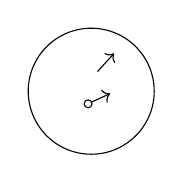
\begin{tikzpicture}[x=1cm,y=1cm]
 \draw (0,0) circle (0.8);
 \draw (-0.04,-0.16) circle (0.05);
 \draw[->] (0,-0.14) -- (0.24,-0.03);
 \draw[->] (0.08,0.25) -- (0.29,0.48);
\end{tikzpicture}
\end{adjustbox}
\end{center}

Или: профакторизовать по max комп. подгруппе

\begin{center}
\begin{adjustbox}{max width=\linewidth}
\begin{tikzpicture}[x=1cm,y=1cm]
 \draw (0,0) circle (1.15);
 \draw (0.05,1.14) .. controls (0.08,0.65) and (-0.01,0.2) .. (-0.39,-0.12);
 \draw (0.05,1.14) .. controls (0.04,0.62) and (0.27,0.42) .. (0.43,0.10);
 \draw (-0.39,-0.12) .. controls (-0.05,0.17) and (0.23,0.17) .. (0.43,0.10);
 \draw (0.045,0.72) -- (0.19,0.66);
 \draw (-0.27,0.02) .. controls (-0.2,0.03) .. (-0.18,0.12);
 \draw (0.32,0.12) .. controls (0.27,0.18) .. (0.30,0.27);
 \node at (0.11,0.52) {$0$};
 \draw (2.8,1.1) .. controls (2.7,0.38) and (2.45,0.02) .. (1.89,-0.32);
 \draw (2.8,1.1) .. controls (2.77,0.48) and (3.11,0.09) .. (3.46,-0.35);
 \draw (1.89,-0.32) .. controls (2.39,-0.12) and (2.98,-0.06) .. (3.46,-0.35);
 \draw (2.69,0.68) -- (2.84,0.7);
 \draw (2.17,-0.16) .. controls (2.29,-0.1) .. (2.30,0.03);
 \draw (3.17,-0.19) .. controls (3.12,-0.10) .. (3.14,0.02);
 \node at (2.78,0.51) {$0$};
 \node at (2.43,0.04) {$\pi/3$};
 \node at (3.04,0.03) {$\pi/3$};
 \draw[->] (4.05,0.49) -- (3.59,0.49);
 \node[anchor=west] at (4.13,0.49) {\underline{фунд. область}};
\end{tikzpicture}
\end{adjustbox}
\end{center}

\underline{Ответ.}
\begin{equation}
 \operatorname{vol}\mathrm{SL}(n,\mathbb R)/\mathrm{SL}(n,\mathbb Z)
 =\zeta(2)\zeta(3)\ldots\zeta(n)
 \tag{2}
\end{equation}
$\mathbb A$ — адели;
\begin{equation}
 \begin{gathered}
 \mathrm{SL}(n,\mathbb A)\sim
 \mathrm{SL}(n,\mathbb R)\times\mathrm{SL}(n,\mathbb Q_2)\times\ldots\\
 \cup\\
 \mathrm{SL}(n,\mathbb Q)
 \end{gathered}
 \tag{3}
\end{equation}
\begin{equation}
 \operatorname{vol}\mathrm{SL}(n,\mathbb A)/\mathrm{SL}(n,\mathbb Q)=1.
 \tag{4}
\end{equation}
\begin{equation*}
 \operatorname{vol}\mathrm{SL}(n,\mathbb A)/\mathrm{SL}(n,\mathbb Q)
 \sim
 \operatorname{vol}\mathrm{SL}(n,\mathbb R)/\mathrm{SL}(n,\mathbb Z)
 \prod\operatorname{vol}\mathrm{SL}(n,\mathbb Z_p).
\end{equation*}
\begin{equation}
 \operatorname{vol}\mathrm{SL}(n,\mathbb Z_p)
 \sim\#\mathrm{SL}_n(\mathbb F_p)/p^{n^2-1}.
 \tag{5}
\end{equation}
\underline{Упражнение}: вычислить $\#\mathrm{SL}_n(\mathbb F_p)$.

\SourcePage{GELFAND-P001421}{unlabelled}
(6) Число элем. $\mathrm{GL}(n,\mathbb F_p)$
\begin{equation*}
 (p^n-1)(p^n-p)(p^n-p^2)\ldots
 =
 p^{n^2}(1-p^{-n})(1-p^{-n+1})\ldots(1-p^{-1}).
\end{equation*}

(7) Для $\mathrm{SL}(n,\mathbb F_p)$ надо поделить на $p-1$:
\begin{equation*}
 p^{n^2-1}(1-p^{-n})(1-p^{-n+1})\ldots(1-p^{-2}).
\end{equation*}
Это произвед. эйлеровых сомножителей.

(8) \underline{Гипотеза Ю.И. Манина}: аналог ф-лы (2) можно написать для
пр-в модулей кривых, возник. в теории струн.

\underline{И.М.Г.}

\underline{Мат. вопрос}: объём пр-ва Тейхмюллера имеет $p$-адический аналог.

Или: что такое адельное пр-во Тейхмюллера

\medskip
\underline{Пример \Unclear{GELFAND-P001421}{witten-heading-faint-word}{силы} работ Виттена:}

\underline{Laumon} сделал раб. по теории чисел на основе идей Виттена
из теории Морса.

Идея: рассм. ф-ю $u\in\mathcal E'(\mathbb R)$,
$\widetilde u(\xi)\in C^\infty$
и все особ. уйдут в асимптотику на бесконечности.

\underline{Совет И.М.Г.}: прочитать книгу Харкевича
«Спектры, [зачёркнуто:
\Unclear{GELFAND-P001421}{book-title-cancelled}{неразборчиво};
вставлено над строкой: сигналы] и шумы»,
чтобы понимать преобр. \underline{Фурье}.

О раб. \underline{Laumon'а}.

\begin{center}
\begin{adjustbox}{max width=\linewidth}
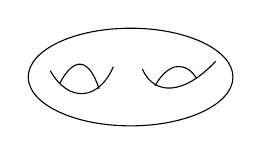
\begin{tikzpicture}[x=1cm,y=1cm]
 \draw (0,0) ellipse (1.3 and 0.62);
 \draw (-1.02,0.08) .. controls (-0.78,-0.34) and (-0.40,-0.29) .. (-0.22,0.13);
 \draw (-0.90,-0.08) .. controls (-0.72,0.26) and (-0.53,0.25) .. (-0.40,-0.15);
 \draw (0.15,0.10) .. controls (0.30,-0.24) and (0.68,-0.23) .. (1.08,0.20);
 \draw (0.31,-0.11) .. controls (0.50,0.22) and (0.72,0.18) .. (0.84,-0.02);
\end{tikzpicture}
\end{adjustbox}
\end{center}

Рассм. поверхность $\mathcal F$
\begin{equation*}
 H^i(X,\mathcal F),\qquad i=0,1,2.
\end{equation*}
\Unclear{GELFAND-P001421}{surface-symbol}{После «поверхность» стоит $\mathcal F$; далее написано $H^i(X,\mathcal F)$.}

\begin{equation}
 \det H^\bullet(X,\mathcal F)=
 \frac{\det H^0(X,\mathcal F)\det H^2(X,\mathcal F)}
 {\det H^1(X,\mathcal F)\;
 \text{[зачёркнуто: }\det H^2(X,\mathcal F)\text{]}}
 \tag{1}
\end{equation}
([Зачёркнуто:
\Unclear{GELFAND-P001421}{before-vector-spaces-cancelled}{конечные?}]
вект. пр-ва;
$\det$ — max внеш. степень)

Автоморфизмы?

Рассм. триангуляцию; $\det H^\bullet$ отожд. с произвед. $\det$
членов комплекса (ф-ла типа Эйлера): канонически

\SourcePage{GELFAND-P001422}{64}
\begin{equation*}
\det(C^\bullet)=\det(H^\bullet(C)) \tag{2}
\end{equation*}
$2-2g$ — эйлерова хар-ка.

С другой стороны
\begin{equation*}
2g-2=\operatorname{deg}K
\end{equation*}
[Под $K$: «кан. класс».]

\underline{Пусть}

$D$ — дивизор;
\begin{equation*}
\det\mathcal F_D=\bigotimes(\det\mathcal F_{x_i})^{\otimes a_i},
\qquad D=\sum a_i x_i \tag{3}
\end{equation*}
[Зачёркнуто:
\Unclear{GELFAND-P001422}{cancelled-divisor-map}{$D\to D+K$ или $D\mapsto D+K$; чтение не установлено}.]

\underline{Ф-ла Делиня:}
\begin{equation*}
\det H^\bullet=\det\mathcal F_K \tag{4}
\end{equation*}
[Справа зачёркнут отдельный знак:
\Unclear{GELFAND-P001422}{eq4-cancelled-sign}{неразборчиво}.]
\Unclear{GELFAND-P001422}{eq4-determinant-convention}{В (4) написано $\det H^\bullet=\det\mathcal F_K$, без показателя $-1$.}

(фиксир. комплексную структуру и выбор точки в кан. классе)

Для произв. конструкт. пучка тоже считается $\underline{\det}$ и
есть аналог ф-лы Делиня!

Здесь на $\mathbb A^1$ возникают ф-и с особенностями

\underline{\underline{Клячко.}}\quad
\underline{\underline{Торические расслоения.}}

Торическое мн-зие — мн-зие $X$ на к-ром действует алг. тор $T$;
причём есть орбита, изом. $T$.
\begin{equation*}
X=\bigcup_\sigma O_\sigma,\quad\text{— разложение на орбиты}
\end{equation*}
$\mathcal E$ — расслоение на $X$ с торической структурой
(и действие поднимается! диагр.
\begin{equation*}
\begin{adjustbox}{max width=\linewidth}
\begin{tikzcd}
\mathcal E \arrow[r,"t"] \arrow[d] & \mathcal E \arrow[d] \\
X \arrow[r,"t"] & X
\end{tikzcd}
\end{adjustbox}
\end{equation*}
коммутативна)

Можно описать модули [вставлено над строкой: «таких»]
расслоений на языке линейной алгебры.

\SourcePage{GELFAND-P001423}{unlabelled}
Строение $X$ описывается веером $\Sigma$ в алгебре Ли тора.
\begin{center}
\begin{adjustbox}{max width=\linewidth}
\begin{tikzpicture}[scale=0.9]
\draw (0,0) -- (-1.65,0.9);
\draw (0,0) -- (-1.45,-0.95);
\draw (0,0) -- (-0.12,1.65);
\draw (0,0) -- (0.15,-1.65);
\draw[->] (0,0) -- (1.05,1.45);
\draw[->] (0,0) -- (1.8,0.9);
\draw[->] (0,0) -- (1.85,-0.5);
\draw (0.36,0.19) -- (0.3,0.42);
\draw (0.64,0.32) -- (0.52,0.72);
\draw (0.95,0.48) -- (0.76,1.05);
\draw (1.28,0.64) -- (1.02,1.33);
\draw (0.35,-0.10) -- (0.43,0.20);
\draw (0.64,-0.18) -- (0.71,0.33);
\draw (0.96,-0.26) -- (1.03,0.47);
\draw (1.29,-0.35) -- (1.35,0.59);
\node at (1.65,1.35) {$\sigma$};
\node at (1.95,0.28) {$\sigma$};
\node at (4.3,0.75) {(конусы)};
\end{tikzpicture}
\end{adjustbox}
\end{center}
$|\Sigma|$ — мн-во $1$-мерных конусов в веере $\Sigma$.

\underline{Теорема.}
(Катег. торич. расслоений) $\Longleftrightarrow$
(катег. вект. пр-в
[зачёркнут знак:
\Unclear{GELFAND-P001423}{theorem-cancelled-sign}{неразборчиво}]
$E$ набором [над строкой вставлено: «убыв. $\mathbb Z$-»]
фильтраций $E^\alpha(i)$, $\alpha\in|\Sigma|$, удовл. условию

А) Фильтрации $E^\alpha$, $\alpha\in\sigma\in\Sigma$,
дистрибутивны.

\underline{Задачи.}
1) Описать геометрию расслоения (когом., хар. классы
и т. п.) на языке фильтраций

2) классификация — ?

Пусть $\Sigma$ — симплиц. комплекс; поставим вершине в соотв.
фильтрацию

Его предст. — набор фильтраций в вект. пр-ве
[вставлено над строкой: «$E$:»] $E^\alpha(i)$,
$\alpha\in$ [зачёркнут знак:
\Unclear{GELFAND-P001423}{representation-cancelled-sign}{неразборчиво}]
$\Sigma$,
\begin{equation*}
E\ldots\supset E^\alpha(i)\supset E^\alpha(i+1)\supset\ldots 0
\end{equation*}
\begin{equation*}
\alpha\in(\text{вершины комплекса})=\Sigma.
\end{equation*}
Пр-ва $E^\alpha(i)$, $\alpha\in\sigma$, дистрибутивны при фиксир. $\sigma$
(для всех $i$)

[Под первым $\sigma$: «симплекс». Вставка в обводке:]
(т. е. порождают дистрибу. решётку)

Напр., если

$\alpha_1,\alpha_2,\alpha_3$ — вершины $\Delta$-ка, то

$E^{\alpha_1}\quad E^{\alpha_2}\quad E^{\alpha_3}$ дистрибутивны, т. е.
\begin{equation*}
(E^{\alpha_1}+E^{\alpha_2})\cap E^{\alpha_3}
=E^{\alpha_1}\cap E^{\alpha_3}+E^{\alpha_2}\cap E^{\alpha_3}
\end{equation*}

\underline{Классифицировать:} хорошая задача

Для тр-ка: решается тривиально

Для поверхности тетраэдра $\Sigma=\partial\Delta$, $\Delta$ — симплекс, ответ
таков: в [зачёркнуто:
\Unclear{GELFAND-P001423}{tetrahedron-cancelled-space}{$\mathbb R^3$-пр-ве; чтение не установлено}]
$E$, $\dim E=3$, рассм. $4$ $2$-мерных подпр-ва общего положения.
\begin{equation*}
\mathcal E=(E;\ E^\alpha,E^\beta,E^\gamma,E^\delta)
\end{equation*}

\SourcePage{GELFAND-P001424}{65}
ещё нужно взять внешние степени
\begin{equation*}
\Lambda^i\mathcal E=
(\Lambda^i E,\Lambda^i E^\alpha,\Lambda^i E^\beta,
\Lambda^i E^\gamma,\Lambda^i E^\delta)
\end{equation*}
Общее предст. разл. в прямую сумму $1$-мерных и таких.

\underline{И. М. Г.}
Правильная задача: выделить в $\forall$ задаче разрешимые
куски (идеология Гельф.-Пономарева)

У В. [исправленный и зачёркнутый инициал:
\Unclear{GELFAND-P001424}{kac-initial}{неразборчиво}]
\underline{Каца} всё это описано на языке графов и алгебр
\underline{Каца-Муди}:
размерности вершин = коорд. корней и т. п.

Находится число параметров.

Lect. Notes, \underline{996}; более ранняя раб. — \underline{Inventiones}.

(докл. на конференции)

[Зачёркнута строка:
\Unclear{GELFAND-P001424}{cancelled-seminar-line}{Семинар \ldots; остальное неразборчиво}.]

\Incomplete{GELFAND-P001424}{cancelled-seminar-content}{Полное чтение зачёркнутой строки перед «След. раз: 8 февраля» не установлено; возможное начальное слово приведено выше.}

\underline{След. раз:}\quad \underline{8 февраля.}



\end{document}
